\documentclass[main.tex]{subfiles}
% \nomenclature[A]{GPR}{Ground Penetrating Radar}%

\begin{document}
\begin{appendices}
\addtocontents{toc}{\protect\setcounter{tocdepth}{0}}

\chapter{Benchmarking}
\chaplabel{benchmarking}
\textcolor{red}{If you have time, make this section broader (more benchmarking against platforms like the Husky, )} Before commencing the design process, benchmarking was conducted in order to gauge the capabilities of existing platforms and sensor equipment used for landmine detection. This gave an indication of the minimum requirements to be set for the project, and helped to better understand what challenges would need to be overcome.

\section{Autonomous platforms for landmine detection}
The use of a vehicle for landmine detection allows for larger areas to be scanned in a shorter period of time. Vehicles can also support greater loads than any human operator could, which means that more sensing equipment can be carried; this in turn increases sensing capability, and reduces the likelihood of false positives. If the vehicle can operate remotely or autonomously, the risk to human operators can be eliminated entirely. For these reasons, remotely controlled or autonomous platforms have become a popular tool for landmine detection. This section looks at several such platforms that are currently in operation or in development. 

%\subsection{Landmine detection vehicles}

In military scenarios, the key priority is to clear a path as quickly as possible for a convoy \parencite{portugal2014}. In many cases, landmine detection is coupled with landmine clearance. On the other hand, humanitarian demining requires greater levels of accuracy and effort. A clearance rate of 80\% is generally accepted in combat, a figure which only needs to apply to pathways where troops or convoys will travel; for humanitarian situations, the area required to be cleared is much larger, and such a low clearance is not accepted \parencite{habib2008}. \Figref{military} shows two remotely controlled landmine detection vehicles, one of which is used in military operations, while the other is commercially available for humanitarian demining.   

\begin{figure}[ht]
\centerline{
\begin{tabular}{cc}
\subfloat[FORESIGHT RDV \parencite{canada2004}]{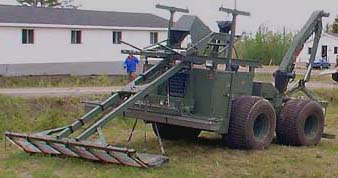
\includegraphics[height=0.25\textwidth]{8-Appendices/foresight.jpg}}
& \subfloat[NIITEK Minestalker \parencite{niitek2015}]{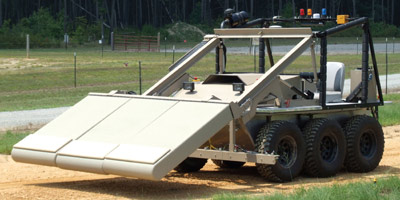
\includegraphics[height=0.25\textwidth]{8-Appendices/minestalker.jpg}} \\
\end{tabular}}
\caption{Military and commercially available vehicles for landmine detection}
\figlabel{military}
\end{figure}
 
\subsubsection*{General Dynamics FORESIGHT RDV} 
FORESIGHT is a multi-sensor landmine detection system, mounted on a vehicle that can be controlled remotely. The vehicle usually travels with a protection vehicle, which clears the the path ahead of surface-based devices, as well as mines just below the surface \parencite{canada2004}. The sensor suite consists of four independent systems, the data from which is fused to accurately detect a range of threats. A minimum metal detector array which is 3 m wide is used for the detection of metallic parts, even when the metal content is low. The 3 m GPR array with ultra-wide band capabilities (1-3 GHz) can detect larger mines at up to 30 cm below the soil surface. An infra-red camera with 8-14 micrometre wavelength is used to detect changes in soil density which occur when mines are buried \parencite{canada2004}. Finally, a thermal neutron activation detector directly detect explosives through measurements of the soil nitrogen level; this provides an added level of target confirmation \parencite{general2009}. The sensor suite can operate at a forwards speed of 3-4 km/h, and in the event that a detection is made with a sufficient confidence level, the onboard marking system is used to physically mark the threat location \parencite{canada2004}.

\subsubsection*{NIITEK Minestalker} 
Developed by the US Department of Defense and NIITEK for humanitarian demining, the Minestalker system was built to detect anti-tank mines at depths greater than 5 to 10 cm \parencite{laudato2014}. The system utilises a high performance 3.2 m VISOR GPR array and optional 3 m See-Deep metal detector array \parencite{niitek2015}. The sensors are mounted on a tractor vehicle which can be controlled remotely; the accompanying software system ensures that there is a high detection probability and a low number of false alarms. The system is a "user in the loop system", in the sense that the vehicle stops when a target is detected and waits for further instructions \parencite{laudato2014}. Targets are marked both physically and with GPS, with a 1 metre resolution. The vehicle itself can advance and detect threats in real time at up to 15 km/h \parencite{niitek2015}.

% \subsection{Research Vehicles}
% While commercially available vehicles for landmine detection are often modelled on military vehicles, research vehicles are much more varied in their design (\Figref{research}). These vehicles have been developed by universities or other research organisations, and in most cases have not seen any operational use.

% \begin{figure}[ht]
% \centerline{
% \begin{tabular}{cc}
% \subfloat[Clearpath Husky \parencite{hennessey2014}]{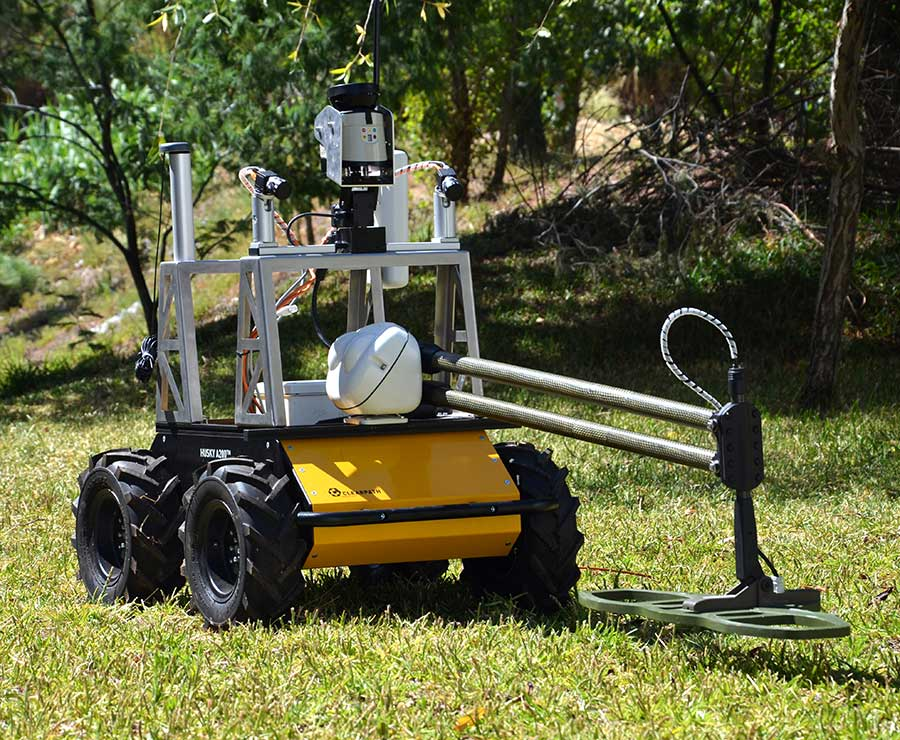
\includegraphics[height=0.3\textwidth]{8-Appendices/clearpath.jpg}} 
% & \subfloat[SILO6 \parencite{santos2007}]{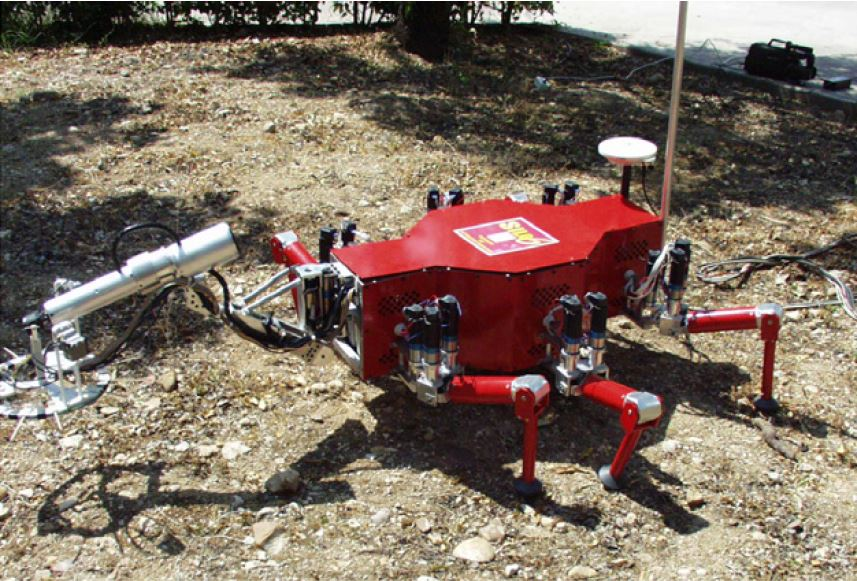
\includegraphics[height=0.3\textwidth]{8-Appendices/silo6.jpg}}\\
% \subfloat[tEODor \parencite{cubber2014}]{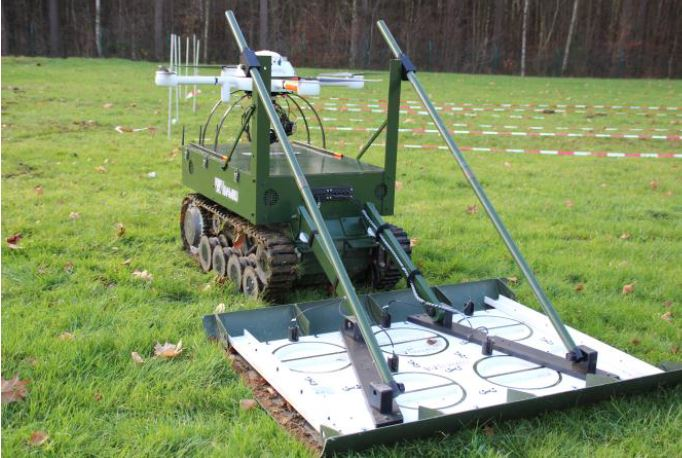
\includegraphics[height=0.3\textwidth]{8-Appendices/teodor.jpg}} 
% & \subfloat[Gryphon \parencite{fukushima2008}]{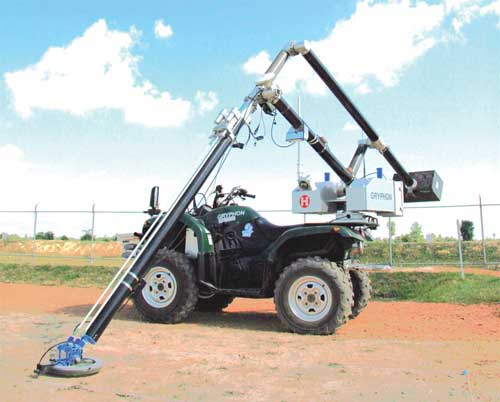
\includegraphics[height=0.3\textwidth]{8-Appendices/gryphon.jpg}}
% \end{tabular}}
% \caption{Research vehicles for landmine detection}
% \figlabel{research}
% \end{figure}

% \paragraph{Clearpath Husky} The Husky is an autonomous vehicle produced by Clearpath Robotics. In 2012, a team at the University of Coimbra (Portugal) used this platform as  foundation to create a landmine detection vehicle \parencite{hennessey2014}. The sensor suite consists of a metal detector on a robotic arm, and a GPR. The Husky itself has autonomous capabilities, meaning it can complete a mission without operator interaction \parencite{portugal2014}. The vehicle has an operational speed of 1 m/s, with an operating time, limited due by the battery life of the Husky, of 3 hours. 

% \paragraph{SILO6} SILO6 is a six-legged landmine detection robot. The six legs allow it to better traverse rough terrain, and increase mobility; in order to increase stability, the robot can lower its centre of gravity by bending its legs \parencite{santos2007}. The robot is semi-autonomous, however it has a limited sensor capability. The only sensor currently used is a Schiebel AN-19/2metal detector, which is capable of detecting objects with a low metal content. The design of the platform restricts the operating speed to 0.5 m/s, with a typical speed of 0.1 m/s, while the maximum operating time is 1 hour \parencite{portugal2014}.  

% \paragraph{tEODor} The tEDOor platform is a tracked, remotely controlled vehicle that is commercially available for the disposal of explosive ordnance. The platform was heavily modified by the Royal Military Academy (Belgium) to assist in humanitarian demining \parencite{cubber2014}. A metal detector array is fitted to the front of the platform, which is able to detect both small and large mines. The system works in conjunction with an unmanned aerial vehicle, which firstly scans the area using visual and infra-red sensors, and identifies points of interest which tEODor investigates. Being a tracked vehicle, the operating speed is limited, in this case to a maximum of 0.8 m/s, while the operating time is 203 hours \parencite{portugal2014}.   

% \paragraph{Gryphon}
% The Gryphon project is larger in scale than the rest of the research projects introduced. It uses a commercially available quad bike on which a large arm has been fitted \parencite{fukushima2008}. The length of the arm allows the vehicle to remain completely outside of the test lane, meaning this it is less susceptible to damage. A metal detector or GPR can be fitted to the end of the arm, though not at the same time. Since the platform is a larger vehicle, is can be operated at speeds of up to 5 m/s, and the petrol engine allows a 10 hour operating time \parencite{portugal2014}.  

% The various vehicles introduced show that there are many approaches to automated landmine detection, both in terms of the platforms used and the sensors available. While many solutions exist, no one method can be adapted to all scenarios, and there is much room for innovation and further research. \textcolor{red}{Need to speak about the challenges that are present}

%\section{Landmine Detection}
%There have been similar projects that have used MD, GPR or a  combination of both to achieve detection and classification of landmines or unexploded ordinances (UXO). The various models of MD, GPR will be compared in order to determine if the specific details are suitable for landmine detection and if the scenario of operations (\textcolor{red}{insert reference to scenario of operations}) are achievable based on these specifications. 

% \subsection{Metal Detectors}
% \textcolor{red}{Insert some benchmarking here that Rahul did}

% \subsection{Ground Penetrating Radar}
% \textcolor{red}{Need to relate to the scope as well, i.e. soil types and operational environments\\}
% What has been achieved with the GPR in terms of the operation environment and soil types. etc. that can be linked and based on

%In order to meet the system requirements \textcolor{red}{(insert reference to system requirements here)} and  scenarios of operation of the landmine, there are operating parameters required. The operating specifications of a GPR for landmine detection are listed as follows \textcolor{red}{insert Pasolli reference here}:
% \begin{itemize}
% \item{\textbf{frequency:} 10 MHz - 3 GHz}
% \item{\textbf{Penetration depth:} 1 cm - 3 m.}
% \item{\textbf{Surface types:} Sand, humus soil}
% \item{\textbf{Operating time:} 1 ns to 60 ns}
% \item{\textbf{No. of data scans:} 200 - 600}
% \end{itemize}

%The following comparisons of specific GPRs that may be used in landmine detection should meet or exceed the specifications above. There are various types of commercial GPRs, such as NIITEK, SIRO-Pulse, and others as provided below. %-Still changing this part. 

%\paragraph{NIITEK GPR}
%AS provided in landmi
%\paragraph{SIRO-Pulse}

%\paragraph{DX Antenna Array GPR} This type of GPR meets the operating criteria above as specified in \textcolor{red}{see appendix}. There are various applications that this GPR may be used including archaeology,

%The detection of subsurface objects is one of the main uses for a GPR. This concept may be used in various applications including landmine detection. The GPR is able to detect landmines with various types of casing. An advantage of the GPR sensor is that there are both handheld and array types which assist in both manned and unmanned landmine detection operations. There are two types of GPRs, namely pulse radar (time-domain) and frequency-domain \textcolor{red}{specific reference here}. 

%In order detect and identify the subsurface objects as mentioned in \textcolor{red}{reference objective section}, the GPR signals are required to be processed. There are various methods implemented to detect landmines using GPR \textcolor{red}{INSERT CITE}. The first part is the preprocessing of the signals in order to remove signal clutter. This is processed further in order to identify the object under the surface and minimise false positives.

%The detection and classification of landmines and subsurface objects are achieved through existing algorithms, such as, hough transformation, bayesian, feature extraction, kalman filters.   

%\textcolor{red}{NOTE: Need to mention anything commercialised here. Types of GPR used, and the operation frequency they used. The penetration depth etc. etc. Nothing too specific. Just how they've done it. Elaborate on the types in Literature review.} \textcolor{green}{perfect. this is exactly what i was going to put in here - i had a spreadsheet on the GoogleDrive with most of this data in it, but it seems to have gone walkabout}

% Need to check everything
%NOTE NO PHYSICAL MARKING OF THE LANDMINE
%It is also possible to detect the composition of the explosives used in the landmines, however, this is only used in conjunction with the electromagnetic properties returned to receive the signals. 

%Link to Challenges in identifying the landmine due to background noise etc. 
% Need to mention that a database for identification is generally difficult to achieve with regards to current mines. Limitation include that the objects have similar reflected signals, such as rocks vs composite landmines. 

% Need to talk about the usefulness of the GPR and landmine together. How they complement each other. 

\section{Capabilities of landmine detection equipment}
Current mine sweeping methods that employ handheld metal detectors achieve high rates of detection for subsurface metallic mines. The main limitations of the handheld metal detecting systems is the inability to detect mines constructed from non-metallic composite materials, and the shallow depth capabilities provided by the metal detector. These systems also have a high rate of false positives due to the inability for an operator to differentiate between mines and shrapnel fragment or other buried metal objects.

Handheld mine detection devices currently used by the ADF for military purposes include the Minelab F3 series. This device is used to clear paths for vehicles by tracking the wheelbase and scanning for anti-vehicle mines. It has a sensing depth suitable to allow the detection of almost all anti-tank and anti-personnel mines that will pose a threat to an operator, though it has the expected high rate of false positives \parencite{minelabF3}. The process for determining which items are suspicious and require excavation, and which items are unremarkable shrapnel, is required to be undertaken by a skilled operator.
\begin{figure}[ht]
\centerline{
\begin{tabular}{cc}
\subfloat[Minelab F3 \parencite{minelabF3}]{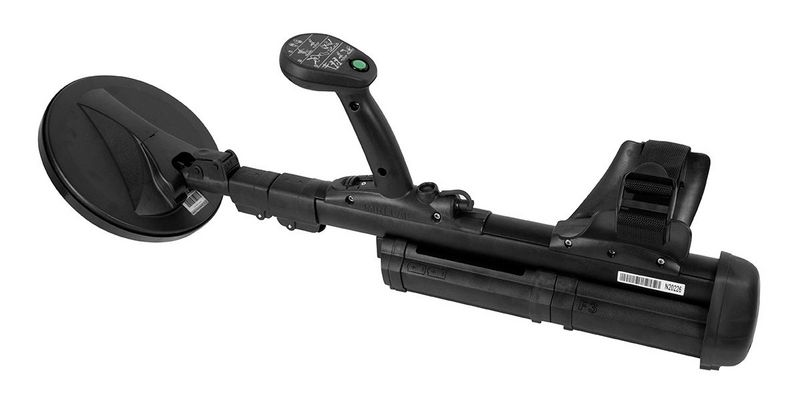
\includegraphics[width=0.5\textwidth]{8-Appendices/minelabF3.jpg}} 
& \subfloat[Minelab STMR \parencite{minelabArray}]{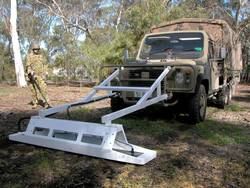
\includegraphics[width=0.4\textwidth]{8-Appendices/stmr.jpg}}\\
\end{tabular}}
\caption{Minelab metal detector systems used by the ADF \& DSTG}
\figlabel{metaldetectors}
\end{figure}

Minelab also provides the STMR, a vehicle mounted metal detection array that reduces the need for on-foot operators in front of a convoy. The sensor is capable of sampling at a rate of 200 Hz, meaning that the device can detect objects while moving at speeds up to 50 km/h \parencite{3dradarDXG}. Like the F3 series, the STMR is capable of detecting minimum-metal mines, such as the composite M14 anti-personnel mine, which contains only a small button sized metal detonator in the entire device \parencite{minelabArray}. The STMR system provides some level of feature recognition, providing a display to the operator inside the vehicle which reports scanned data \parencite{minelabArray}.

Commercially available GPR systems are commonly intended for non-mine detection purposes, such as utility and buried pipe detection. The limitations of 2D radar systems, which include the majority of available GPR devices, is that the narrow scan width means that the antenna is required to pass directly over the mine object to register a detection. A typical scan deviance from the buried object to still consistently register a detection is approximately 150 mm \parencite{3dradarDX}.

Commercial 2D GPR systems range from handheld devices which are intended to detect utilities and locate studs in wall cavities, such as the RadioDetection RD8000, have detection depths of only a few centimetres and limited resolution \parencite{rd8000}. More advanced systems with limited depth ranges, such as the US Radar Seeker 2000 HH are capable of detection resolutions to allow identification of a fishing line at depths of 0.6 metres \parencite{usradar}. The ability to consistenty locate features this small are limited by the signal to noise ratio, a property of the soil in which the search is undertaken. Typical limits for detection capabilites of these GPR units range from a few centimetres to many metres in depth, with reduced resolution as depth of scanning increases.
\begin{figure}[ht]
\centerline{
\begin{tabular}{cc}
\subfloat[RadioDetection RD8000 \parencite{rd8000}]{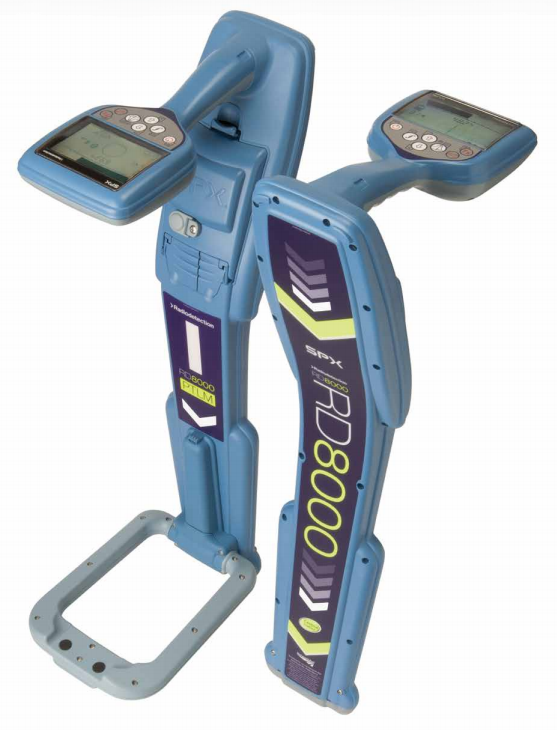
\includegraphics[height=0.4\textwidth]{8-Appendices/rd8000.png}} 
& \subfloat[US Radar Seeker 2000 HH \parencite{usradar}]{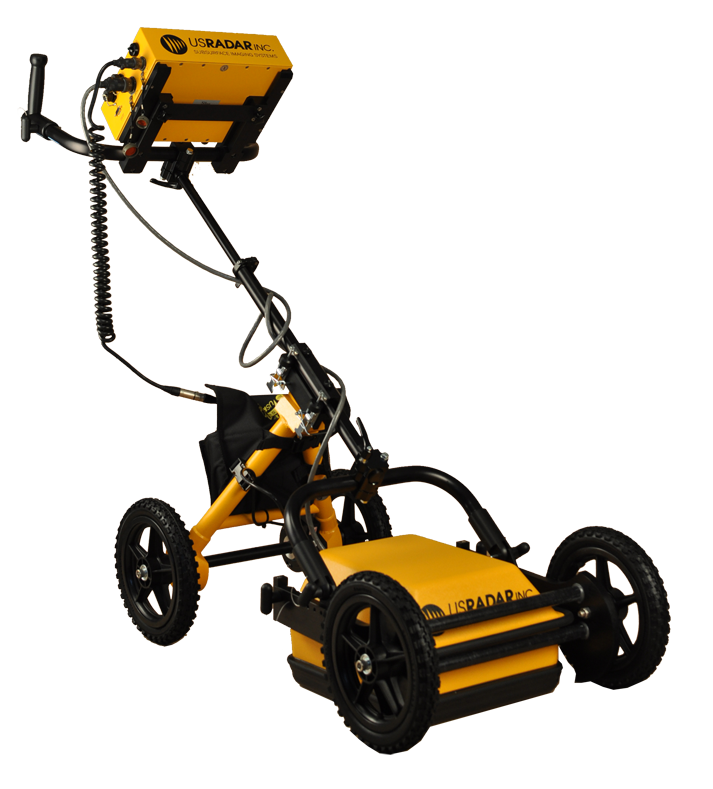
\includegraphics[height=0.4\textwidth]{8-Appendices/seeker2000.png}}\\
\end{tabular}}
\caption{Commercially available GPR systems}
\figlabel{cheapradar}
\end{figure}

A common theme among these systems is limited ability for automatic classification of targets. The large majority require a skilled operator to identify all targets and provide no degree of automatic scanning. More advanced and expensive units offer greater software capabilities for data logging and feature identification, though due to their multi-purpose nature are not capable of providing a high degree of mine detection and identification autonomously with software \parencite{rd8000}.

Current state-of-the-art GPR systems for mine detection, such as the DX and DXG series detectors from 3D-RADAR AS have significantly greater detection capacity than other GPR systems. The DX series, which are specially designed for detection of landmines and unexploded ordnance (UXO) is capable of achieving high detection rates (>95\%) of underground mines due to its high resolution. Detection of objects down to 25 mm in feature size, and at depths of over one metre is commonly achieved \parencite{3dradarDX}. The 3D arrangement of the sensors allows for a wide scanning width making it well suited for mine sweeps ahead of a vehicle. The sensor is capable of being trailer mounted and can produce useful data at speeds of up to 30 km/h \parencite{3dradarDX}.

\begin{figure}[ht]
\centering
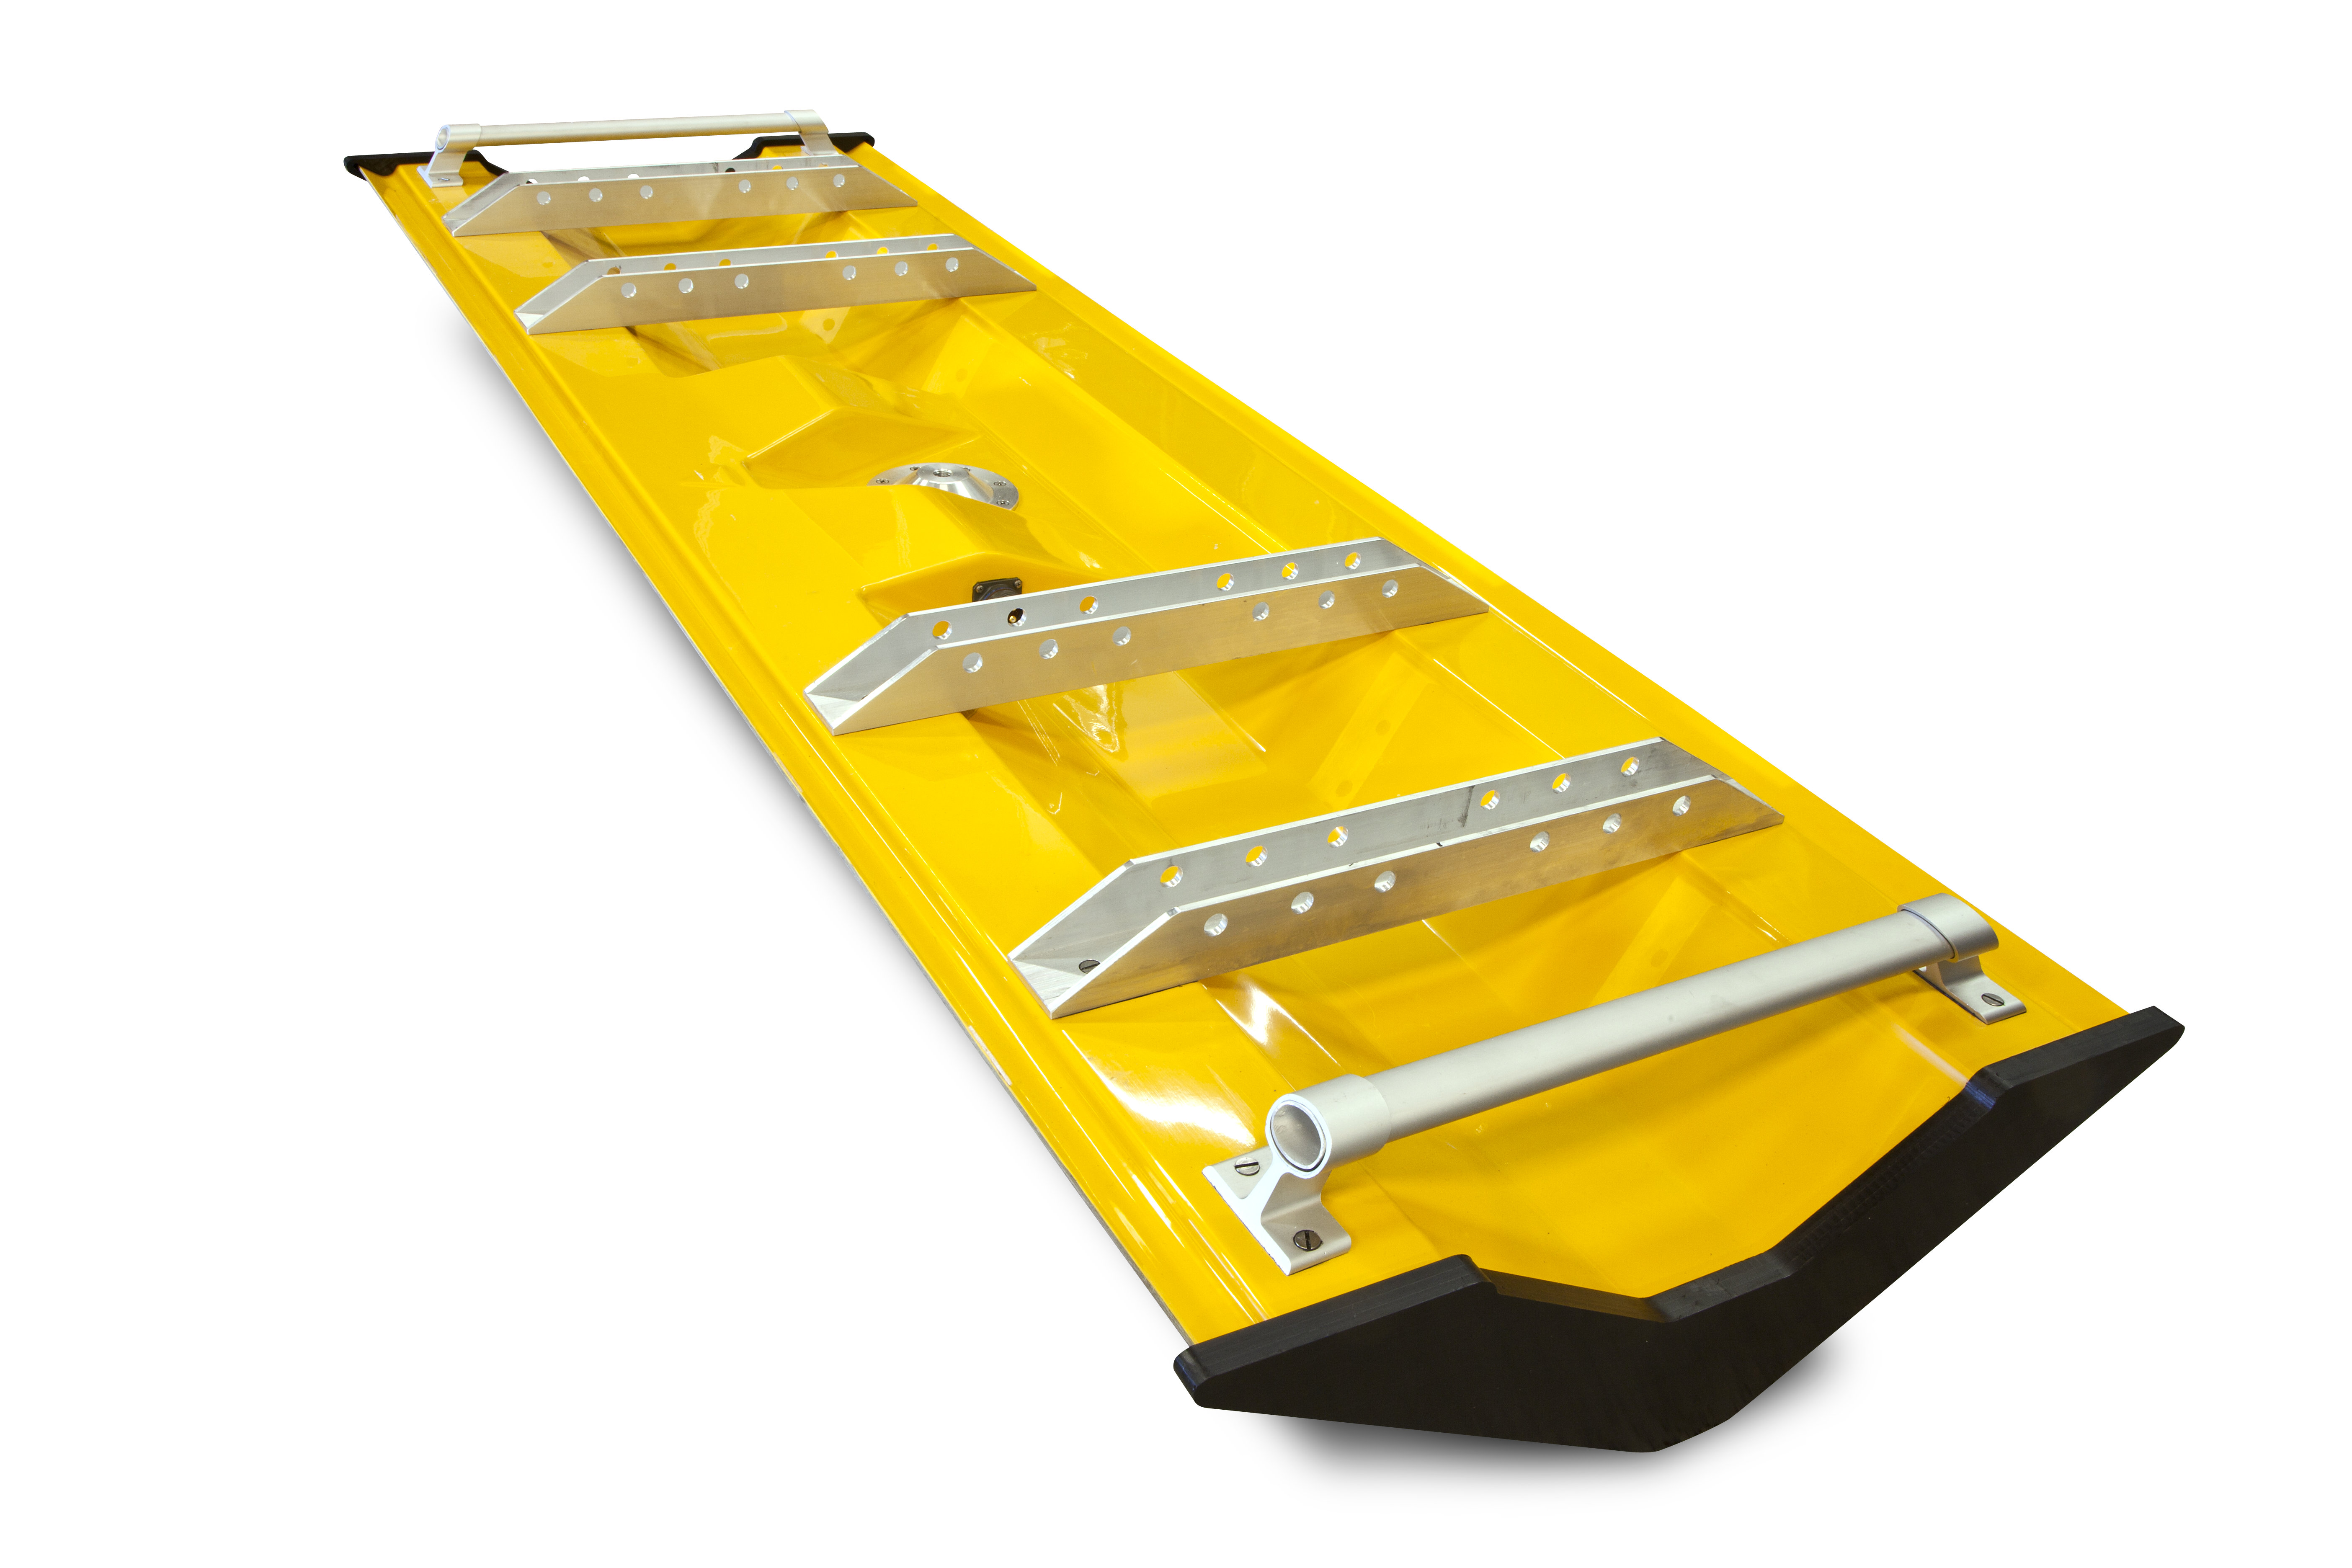
\includegraphics[width=0.55\textwidth]{8-Appendices/DX-Series-Antenna-Profile.jpg}
\caption[3D-RADAR DX series GPR antenna]{3D-RADAR DX series GPR antenna \parencite{3dradarDX}}
\figlabel{dxseries}
\end{figure}

\section{Multisensor systems for landmine detection}
While traditional systems for landmine detection make use of a single sensor, the latest generation of systems attempt to combine multiple sensors. This allows for a broader range of threats to be detected, and at the same time increase detection accuracy.  

% There is no benchmark here so no point talking about it
%\paragraph{AN/PSS-14} The AN/PSS-14, formerly known as the Handheld Standoff Mine Detection System (HSTAMIDS), is the standard mine detector used by the US army since 2006 \parencite{L32012}. The system combines a ground penetrating radar with a metal detector and is designed to detect both anti-tank and anti-personnel mines. The wide-band GPR has a single transmit and two receive antennas, and forms the central part of the sensor head, while the metal detector coil sits around the GPR. Sensor fusion allows data from both sensors to be used in threat detection, which maximises probability of detection of the system while minimising the false alarm rate. In addition, the AN/PSS-14 system makes use of a real-time terrain model, which allows for optimal operation in varying soil conditions \parencite{L32012}. 

One such example is the Vallon Minehound, a commercially available handheld detector that combines a Vallon metal detector with a Cobham GPR \parencite{WM2016}. While the system is designed to find anti-tank and anti-personnel mines, it can also detect low metal content threats such as IEDs. 
%The metal detector employs pulse induction detection to find threats even in soils with a high mineral content, and can be used either independently or in conjunction with the GPR. 
%When used in conjunction, metallic clutter may be ignored, and non-metallic threats can be found. 
System performance in average soil condition allows for detection at depths up to 20 cm for anti-personnel and 40 cm for anti-tank mines, with an overall false alarm rate less than 25\% \parencite{daniels2005}.

Another system is being developed to allow demining and reclamation of vast swathes of currently unsafe land in rural Egypt, where remnants of World War II still pose a significant risk to local communities. The challenge of the Egyptian sands is that the frequently shifting ground surface means that mines are periodically uncovered or more deeply buried than when originally placed many decades ago \parencite{NATOnewsroom}. The system developed combines a highly sensitive metal detector, capable of recognising metallic objects buried at depths greater than a metre, with a GPR which is used to determine the shape and volume of objects located by the metal detector \parencite{NATOnewsroom}. This arrangement allows the detection of deep objects and a reduction in the rate of false positives, reducing the frequency of costly deep excavations of harmless shrapnel.


% There is no benchmark here, so no point talking about it
%\paragraph{ALIS} The Advanced Landmine Imaging System, or ALIS, is a Japanese system that can be integrated with an existing metal detector with minimum modification  \parencite{sato2005}. In addition to the audio output produced by the metal detector, ALIS produces a visual image that combines the metal detector signals with GPR images. The GPR used is a 1-3 GHz impulse radar system, and in order minimise the effect on the metal detector coils, it is mounted at the front of the system  \parencite{sato2005} The signals from both sensors are co-located through the use of a camera mounted on the system, which tracks the relative position of each one.


% Link to challenges in integration 

%The current challenges with landmine detection, including further elaboration of each signal processing methods are \textcolor{red}{reference literature review section}. 

%%%%%%%%%%%%%%%%%%%%%%%%%%%%%%%%%%%%%%%%%%%%%%%%%%%%%%%%%%%%%%%%%%%%%%%%%%%%%%%%%%

\chapter{Platform Selection}
\chaplabel{platformSelectionApp}
As stated in the concept design, the requirements for the platform are as follows: 

\begin{itemize}
 \item Payload: The platform should be able to carry a total payload of 100 kg, and must allow for this payload to be mounted.
 \item Terrain traversing: The platform should be able to travel off-road in regions with dry sandy soils and level unobstructed terrain.
\item  Operational speed and acceleration: The platform should be able travel in a straight line, both forwards and reverse, and perform turns while maintaining an operational speed of 5 km/h.
\item Manoeuvrability and controllability: The platform should be manoeuvrable enough to navigate a region of interest, with a smaller turning angle preferred, yet controllable enough that in case of an emergency, it can come to a complete stop from its operational speed in 1 m.
\item Cost and availability: The platform should have a reasonable cost given the project budget of \$16,500, ans should be available for use as early as possible. 
\item Ease of automation: The platform should be sufficiently simple to automate, with a preference given to platforms that have the framework for automation already implemented. 
\item Ease of transportation: The platform should be sufficiently easy to transport from a workshop to a testing locations using a ute or trailer.
\end{itemize}
The following selection process compares several platforms against these requirements, before selecting the most suitable one. 

\section{Utility quad bike}
Quad bikes are designed to operate off-road, and are capable of traversing a wide variety of terrains with very little difficulty. Since they are designed to carry large loads as well as a human operator, utility quad bikes frequently have load limits larger than 100 kg. The turning radius for a quad bike is typically in the range of 3-4 metres, and the braking distance is small, especially at low speeds. Commercial quad bikes can be purchased at a range of prices, however almost all fall comfortably within the budget. The DSTG also offered the use of an autonomous quad bike, which was previously developed at the University of Adelaide \parencite{scheiner2011}. This quad bike, as seen in \Figref{2011quadbike}, is a Honda TRX450r and has a payload capacity of 110 kg. The quad bike was previously fitted with remote control capabilities and is in good working condition, however \textcite{scheiner2011} recommended that some actuators and electronics should be replaced.
\begin{figure}[ht]
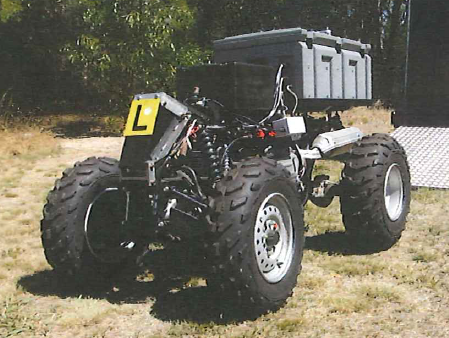
\includegraphics[width=0.5\textwidth]{8-Appendices/2011quadbike.PNG}
\centering
\caption[Autonomous quad bike offered by the DSTG]{Autonomous quad bike offered by the DSTG \parencite{scheiner2011}} \figlabel{2011quadbike}
\end{figure}

\section{Dune buggy}
A dune buggy is a vehicle designed for high speed operation on loose, sandy terrain. Dune buggies are commonly designed with an open chassis housing a modified vehicle and thus its performance characteristics are similar to or better than that of a small car. An example is the Kandi-150 shown in \Figref{kandi150}, which is built to carry two people, allowing for a load capacity exceeding 160 kg. Due to the high speeds at which these vehicles are usually operated, they have turn radii around 6 metres \parencite{150GKM}, restricting path curvature for accurate tracking. Due to the nature of the platform, it would be more expensive than a quad bike and also more difficult to automate.
\begin{figure}[ht]
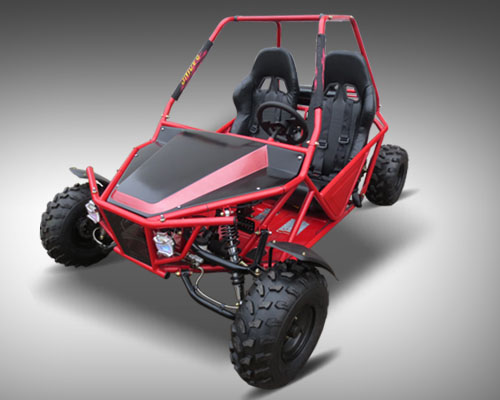
\includegraphics[width=0.5\textwidth]{8-Appendices/kandidunebuggy.jpg}
\centering
\caption[Kandi-150 dune buggy]{Kandi-150 dune buggy \parencite{150GKM}} \figlabel{kandi150}
\end{figure}

\section{Tracked vehicle}
Tracked vehicles are designed to distribute the weight of a vehicle over a large area enabling the traversing of soft and loose terrain without the concern of losing traction and becoming stuck. The platform shown in \Figref{grillon500} is one example of such a vehicle. The Grillon-500 is able to carry a payload of 1000 kg and operate at speeds up to 11 km/h \parencite{cinamGrillon}. This model is designed to support the mounting of various equipment in the front bay (fork lift pictured). An advantage of the tracked vehicle over other platforms is its ability to turn on the spot, eliminating the need for complicated turn algorithms. 
\begin{figure}[ht]
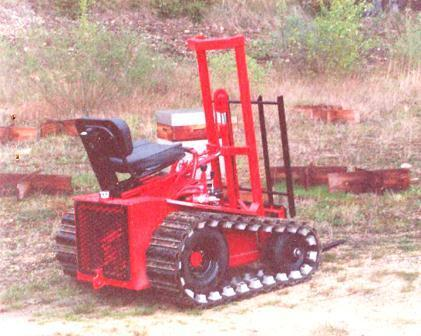
\includegraphics[width=0.5\textwidth]{8-Appendices/Grillon-500.jpg}
\centering
\caption[Grillon-500 tracked vehicle]{Grillon-500 tracked vehicle \parencite{cinamGrillon}} \figlabel{grillon500}
\end{figure}

\section{Hovercraft}

The final platform considered was an existing hovercraft from a University of Adelaide honours project in 2009. Analysis of the technical report \parencite{hovercraft2009} and experimental and theoretical evaluations showed that the lift fan was able to support a payload of up to 22 kg and the thrust fans were only just capable of moving the craft on a flat, smooth surface. Furthermore, it was expected that vibrations produced through the lift and thrust systems on hovercraft platforms would be detrimental to the effectiveness of the sensor equipment. For complete automation, only actuators for the lift motor would be required as remote operation for the thrust system had already been implemented. The stopping distance was lacking due to the time required to rotate fans for reverse thrust. The hovercraft had an advantage over other platforms through its ability to pass directly over a landmine without detonation occurring, however, this 'sliding' advantage introduces new problems when developing a path tracking algorithm due to the advanced dynamics of the platform. This 'sliding' is also a disadvantage is the hovercraft passes over a landmine without detecting it, since it place demining personnel at risk.
\begin{figure}[ht]
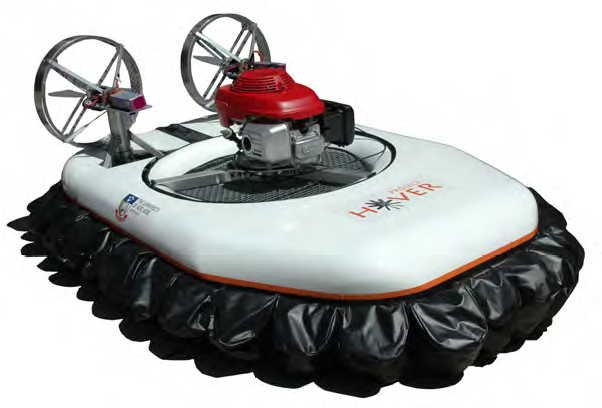
\includegraphics[width=0.65\textwidth]{8-Appendices/HovercraftPic.png}
\centering
\caption[University of Adelaide hovercraft from 2009]{University of Adelaide hovercraft from 2009 \parencite{hovercraft2009}} \figlabel{hovercraftPic}
\end{figure}

\section{Platform decision matrix}
\Tabref{platformDecision} ranks the considered platforms against the platform requirements. The hovercraft was not included due to its inability to meet the minimum payload requirement and poor manoeuvrability. A score of 10 indicates that a certain requirement has been met completely, with lower scores indicating the platform only meets the requirement to a certain extent. 

\begin{table}[ht]
\centering
\caption{Platform decision matrix}
\tablabel{platformDecision}
\begin{tabular}{r *5c}
    \multicolumn{1}{r}{}  & \mcrot{1}{l}{45}{Commercial quad bike} & \mcrot{1}{l}{45}{Dune buggy} & \mcrot{1}{l}{45}{Tracked vehicle} & \mcrot{1}{l}{45}{DSTG quad bike}\\ \toprule 
    Payload & 8 & 7 & 8 & 8\\ 
    Terrain traversing & 9 & 9 & 9 & 9\\ 
    Operational speed and acceleration & 8 & 7 & 10 & 8\\ 
    Manoeuvrability and controllability & 7 & 6 & 9 & 7\\ 
    Cost and availability & 6 & 5 & 4 & 10\\ 
    Ease of automation & 4 & 4 & 5 & 8\\ 
    Ease of transportation & 7 & 7 & 5 & 7\\ \midrule
    \textbf{Total} & 70\% & 64\% & 71\% & 81\%\\ \bottomrule
\end{tabular}
\end{table}

A commercial quad bike or dune buggy could have been used with some modifications to the structure, however a tracked vehicle or the quad bike offered by the DSTG were the two most suitable options. Of these, the tracked vehicle had superior performance specifications, however the DSTG quad bike had the advantage of direct availability at no cost, and an easier path to full automation. Hence, the DSTG quad bike was chosen as the platform for the project. 

%%%%%%%%%%%%%%%%%%%%%%%%%%%%%%%%%%%%%%%%%%%%%%%%%%%%%%%%%%%%%%%%%%%%%%%%%%%%%%%%%%

\chapter{Sensor Mount Material Selection}
\chaplabel{sensorMaterialsApp}
A formal material selection process is undertaken to find the most suitable material for the sensor mount frame, as outlined in \emph{Materials Selection in Mechanical Design} \parencite{Ashby11}. 

\section{Material index derivation}
The first step is to define the problem and find the relevant material index.

\begin{itemize}
\item \textbf{Function}: The sensor mount frame must support loads with negligible deflection and vibration.
\item \textbf{Non-negotiable constraints}: The material used must be non-metallic due to the requirements of the metal detector, and the  frame must have a minimum length $L$, to ensure the sensors are sufficiently far away from the platform.
\item \textbf{Negotiable constraints}: The frame must have a minimum stiffness $E$ equivalent to that of a metal, i.e. stiffness greater than 10 GPa \parencite{Ashby11}, good damping properties, availability and workability, a suitable appearance.
\item \textbf{Objectives}: Minimise mass and vibrations.
\item \textbf{Free variables}: Cost, cross sectional area $A$.
\end{itemize}

The mass $m$ of the frame, assuming a single cantilever beam, is given by $m=AL\rho$, where $\rho$ is the material density. 

For an end loaded cantilever, the bending stiffness $k=\frac{3EI}{L^3}$, where $I$ is the moment of inertia. For a beam with a uniform square cross-section, $I=\frac{A^2}{12}$, which means that $k=\frac{3EA^2}{12L^3}$.

Rearranging and substituting into the mass equation, 
\begin{align}
m=\sqrt{3k}L^{5/2}\big(\frac{\rho}{E^{1/2}}\big).	\eqlabel{mass}
\end{align}

From this equation we can see that to minimise the mass of the frame, we have to maximise $E^{1/2}/\rho$. This material index matches that prescribed by \textcite{Ashby11} for vibration limited designs with length and beam stiffness specified.  

\section{Material selection charts}
Using this material index, material selection charts can be used to identify suitable materials. \Figref{modulus} shows a modulus-density chart, with the dotted lines indicating the stiffness limit of 10 GPa and the minimum mass guideline corresponding to the $E^{1/2}/\rho$ material index. 
\begin{figure}[ht]
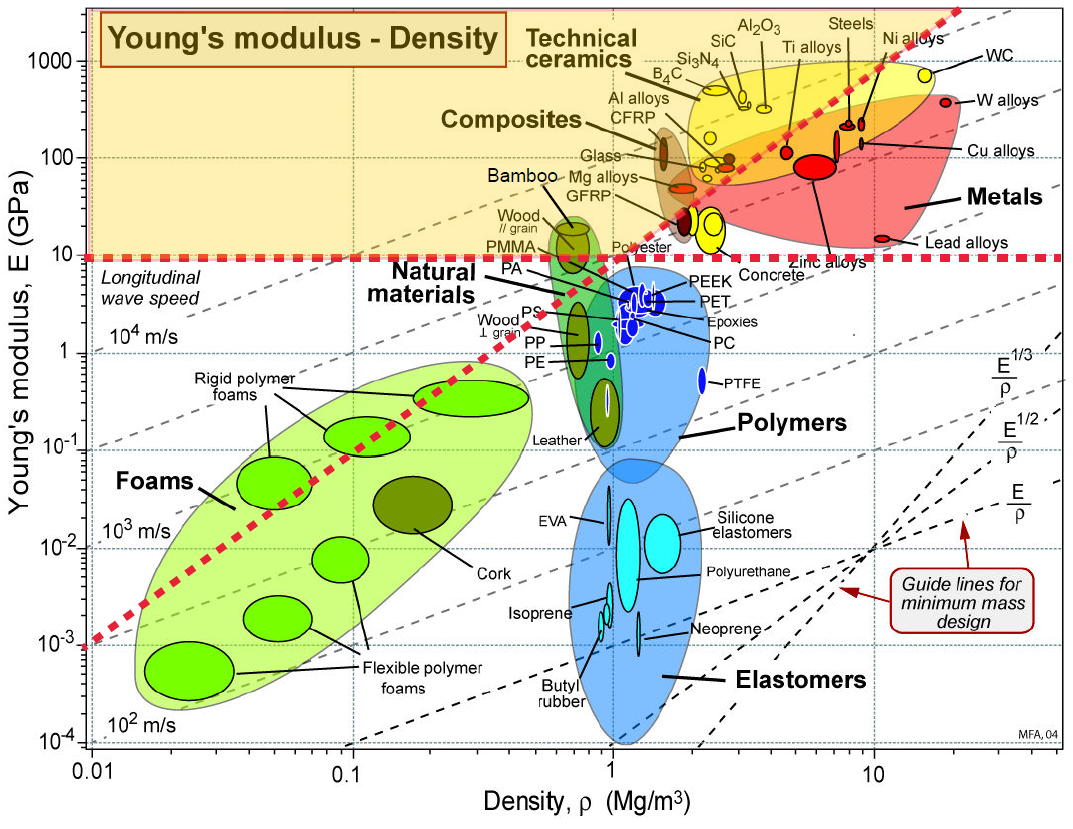
\includegraphics[width=0.9\textwidth]{8-Appendices/modulus.PNG}
\centering
\caption[Modulus-density material selection chart]{Modulus-density material selection chart \parencite{Ashby11}} \figlabel{modulus}
\end{figure}

By shifting the guideline upwards and to the left, the only materials left in the shaded region are some technical ceramics, composites, natural materials and a few metals.
\begin{itemize}
\item Metals: Magnesium and aluminium alloys lie within the region of interest, however they do not meet the non-metallic constraint.
\item Ceramics:  Several ceramic materials such as Al$_2$O$_3$, SiC, and B$_4$C have good stiffness but are heavy and quite difficult to form on account of being brittle. They are also likely to have poor vibrational characteristics.
\item Composites: Carbon and glass fibre reinforced polymers (CFRP and GFRP) have good overall properties, but are expensive and somewhat difficult to form.
\item Natural materials: Bamboo and wood (parallel to grain) also has good properties, they are light but not as stiff as other materials.
\end{itemize}
The most suitable materials are therefore natural materials including wood and bamboo, and composites including CFRP and GFRP.

\Figref{loss} shows a loss coefficient-modulus chart. Of the materials selected previously, bamboo has the highest loss coefficient, followed by wood, GFRP and CFRP, which means it has better stiffness and damping properties. 
\begin{figure}[ht]
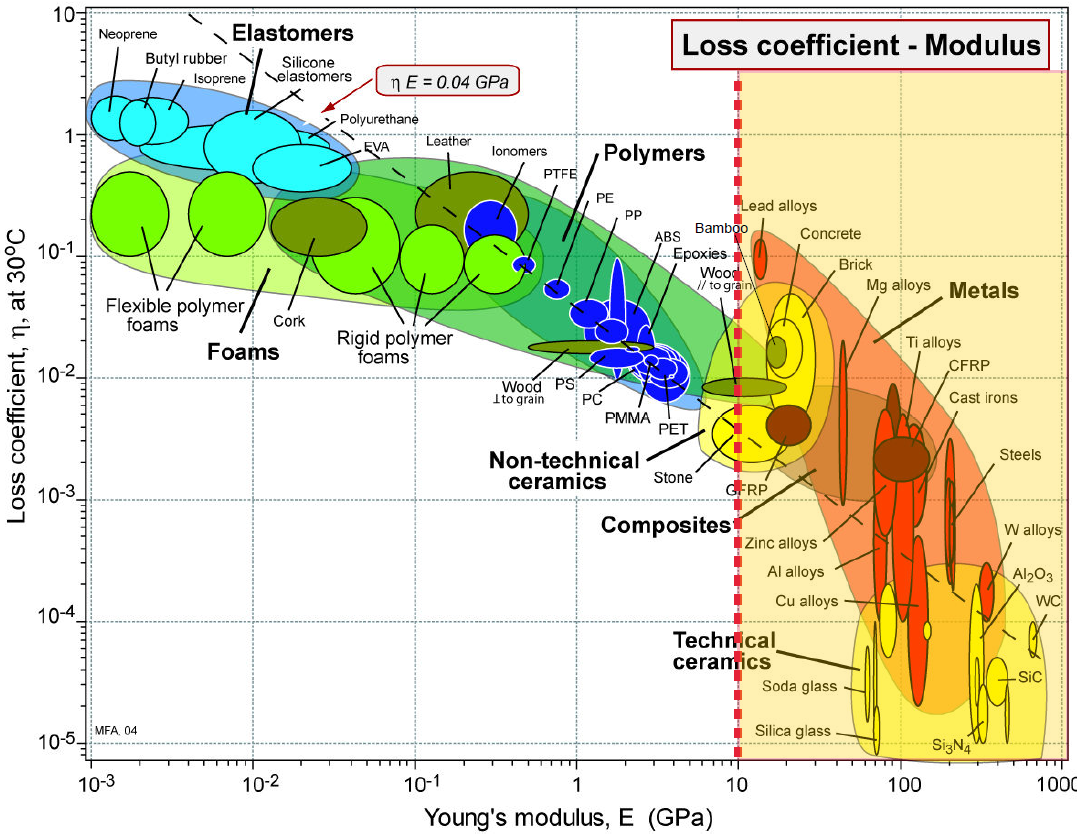
\includegraphics[width=0.9\textwidth]{8-Appendices/loss.PNG}
\centering
\caption[Loss coefficient-modulus material selection chart]{Loss coefficient-modulus material selection chart \parencite{Ashby11}} \figlabel{loss}
\end{figure}

While bamboo is the best material to use for the sensor mount frame based on loss coefficient and stiffness alone, it is difficult to obtain in Australia in structural form. Wood is the next best option, and is very easy to work with and readily available. GFRP has a similar stiffness to wood but with worse damping properties and a higher density. On the other hand, CFRP has a much better stiffness however it sacrifices damping properties and density. The two composites are also more difficult to work with, and are more expensive. Hence, the selected material is wood.

%%%%%%%%%%%%%%%%%%%%%%%%%%%%%%%%%%%%%%%%%%%%%%%%%%%%%%%%%%%%%%%%%%%%%%%%%%%%%%%%%%

\chapter{Steering Selection}
\chaplabel{steeringSelection}
Under the assumption that the quad bike uses the Ackermann steering geometry, i.e. each wheel has it's own pivot during turns, the simplified, 2-wheel model can be used to assess the location of the sensors relative to the quad bike. The simplified model provides the following geometric relationship,
\begin{align}
\tan(\delta) = \frac{L}{R}.
\end{align}
Here, $\delta$ is the steering angle, $L$ is the wheelbase and $R$ is the radius of the arc that the centre of the rear axle will follow. This simplification has been used to perform simulations on the sensor coverage and sensor element misalignment.
%\nomenclature[S]{$L$}{Wheelbase}%
%\nomenclature[S]{$R$}{Radius of rear axle arc}%
Three simulations were conducted, with the steering axle and sensor position changed in each. The results are shown in Figure D.1, and are discussed below.

\begin{figure}[ht]
\centerline{
\begin{tabular}{ccc}
\subfloat[Trial 1]{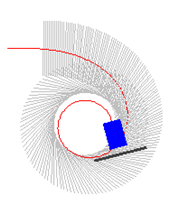
\includegraphics[width=0.3\textwidth]{3-ConceptDesign/Detector_Coverage1.png}}
& \subfloat[Trial 2]{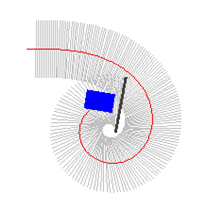
\includegraphics[width=0.3\textwidth]{3-ConceptDesign/Detector_Coverage2.png}}
& \subfloat[Trial 3]{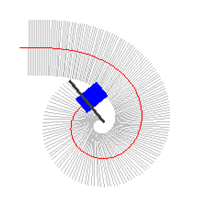
\includegraphics[width=0.3\textwidth]{3-ConceptDesign/Detector_Coverage3.png}}\\
\end{tabular}}
\caption*{\textbf{Figure D.1:} Sensor coverage simulations} 
\end{figure}

\begin{itemize}
\item \textbf{Trial 1}: In first trial, represented in Figure D.1 (a), front wheel steering is used with the sensor mount in front of the platform. The turning wheels are 1.5 metres in front of the focal point of the turn, and the sensor array is 0.5 metres in front of the turning wheels. It is evident from the figure that the coverage area does not form a tight loop, and that this area does not include the path of the vehicle. This is critical as it will mean the quad bike will be passing over ground that has not been scanned by the sensors.
\item \textbf{Trial 2}: In the second trial, represented in Figure D.1 (b), rear wheel steering is used (i.e. the quad bike is using front wheel steering in reverse) with the sensor mount at the front of the platform relative to the direction of travel (i.e. to the rear relative to the actual quad bike geometry). The turning wheels are 1.5 metres behind the focal point of the turn, and the sensor array is placed 0.5 metres in front of the focal axle. This trial shows a much tighter scanning loop than the previous test, and the path of the quad bike is entirely within the scanned area, which is the ideal case.
\item \textbf{Trial 3}: The third trial, represented in Figure D.1 (c), shows front wheel steering with the sensor mount placed behind the front wheels. The turning wheels are 1.5 metres in front of the focal axle as in Trial 1, but the sensing array is 1.5 metres behind the turning wheels, or between the two axles of the vehicle. Under this arrangement, an identical scanning path to Trial 2 is achieved using front-wheel steering, however this is not very useful since the wheels will pass over the region to be scanned before sensors.
\end{itemize}

This result can be demonstrated theoretically by using the geometric bicycle model \parencite{snider2009}. Referring to \Figref{geometricBicycleModel}, the turning radius of the rear wheel is $R$ and the turning radius of the front wheel is $\sqrt{R^2 + L^2}$, which is greater than $R$. If the sensor array was some distance $q$ in front of the front wheels, its turning radius would be $\sqrt{R^2 + [L+q]^2}$, greater yet again. However, if the sensing array was an equal distance $q$ behind the rear wheels (or front wheels if this was a rear steering arrangement) then the turning radius of the sensors would be $\sqrt{R^2 + q^2}$. From this it can be seen that to minimise the effective turning radius then $q$ should be minimised, i.e. rear wheel steering should be used. 


\chapter{Path Subdivision Detail}
\chaplabel{pathSubdivisionDetail}
The path subdivision algorithm cycles through the user or region defined path completing two stages of subdivision at each point.
\begin{enumerate}
\item Subdivide the straight line segment up to the next point
\item If there is a following line segment, conduct a turn and align with it
\end{enumerate}
For the point $P_1 = (x_1, y_1)$, we first subdivide the line segment to the next point $P_2 = (x_2, y_2)$, shown in step 2 of \Figref{simpleTurnProgression}. This is done by doing a linear interpolation between the two points to find a series of intermediate waypoints $P_i = (x_i, y_i)$:
\begin{align}
P_i = |P_2 - P_1| \times k \times j
\end{align}
where $k$ is the distance between intermediate waypoints and j is incremented from 0 to completion of the line segment.
\begin{figure}[ht]
\centering
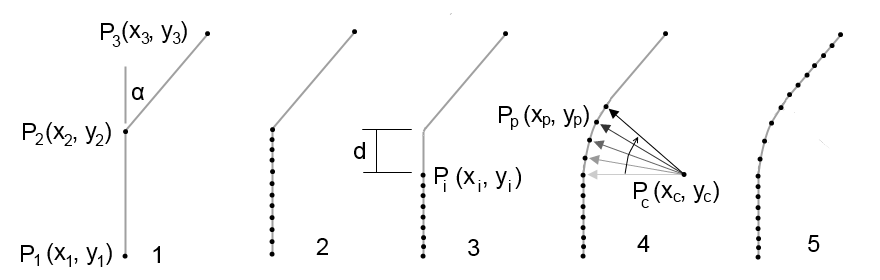
\includegraphics[width=0.9\textwidth]{8-Appendices/simpleTurnProgression.png}
\caption[Simple turn progression]{Simple turn progression}
\figlabel{simpleTurnProgression}
\end{figure}
For a simple turn, a number of intermediate points from the first line subdivision are removed up to a distance $d$ from the turn point, $P_2$. Where
\begin{align}
d = R \tan \frac{\phi}{2}
\end{align}
from \secref{turningspecifiedangle}. The centre point of the turn circle can then be found based on the last intermediate waypoint, $P_i$, and a vector perpendicular to the current path segment with a length equal to the turn radius, 3.14m. The vector is then incrementally rotated around $P_c$ to give the correct distance between waypoints. The required change in rotation angle at each increment is given by the following formula:
\begin{align}
\Delta \textrm{angle} = \frac{\textrm{distance between turn waypoints}}{\textrm{turn radius}} = \frac{0.2}{3.14} = 0.064\ \textrm{rads}
\end{align}
Incrementing stops once the vector has been rotated by a total angle equal to $\phi$. The subdivision process then continues from stage 1, by linearly subdividing the path from $P_2$ to $P_3$.

In the event of a large turn angle where an N-point turn is required, only stage 2 of the subdivision process is changed. Once the linear interpolation of waypoints is complete, some waypoints are either added or removed to the end of the line segment to aid in the alignment of the turn with the next line segment. 
\begin{figure}[ht]
\centering
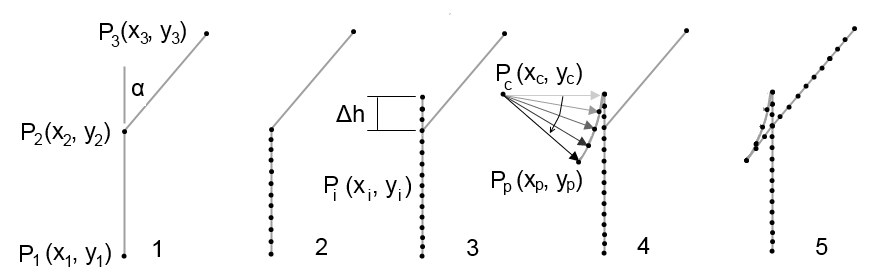
\includegraphics[width=0.9\textwidth]{8-Appendices/nPointTurnProgression.png}
\caption[N-point turn progression]{N-point turn progression}
\figlabel{nPointTurnProgression}
\end{figure}
The distance added or removed, $\Delta h$, is based on the turn angle and is found from the geometrically determined template, Table E.1, shown below.
\begin{table} [ht]
\centering
\caption*{\textbf{Table E.1:} N-point turn template}
\begin{tabular} {r c c c c c c c c}
\toprule
Turn point & 0 & 1 & 2 & 3 & 4 & 5 & 6 & 7 \\ \midrule
Heading (\degree) & 0 & 26.7 & 60.5 & 77.3 & 95.6 & 113.9 & 130.8 & 180 \\
$\Delta h$ required (m) & 0 & 1.46 & 0.09 & 0.44 & 0.37 & 0.11 & 0.62 & -1.18 \\ \bottomrule
\end{tabular}
\end{table}
Similar to the simple turn, the centre point, $P_c$, of the turn arc is be found based on the turn radius, $R$, and is perpendicular to the current line segment. Arc points are added by incrementing the vector by $\Delta \textrm{angle}$. Incrementing stops once the vector has been rotated by a total angle equal to the difference between the current turn point and the next turn point, in the case of \Figref{nPointTurnProgression} part 4, we are at the first turn point so the vector is rotated, $(26.7 - 0)\degree = 26.7\degree$, in total. If at this point the desired turn angle has not been reached, additional arcs are added to the path in the same fashion as just described. Stage 1 is then executed again for the next straight line segment.

\chapter{Extended Kalman Filter Derivation}
\chaplabel{positionDerivation}
The Extended Kalman Filter (EKF) is defined as follows:
\begin{align}
\shortintertext{Prediction Equations:}
&\bar{\mu_t} = g(u_t, \mu_{t-1}) + \delta_t\\
&\bar{\Sigma_t} = G_t\Sigma_tG_t^T + R_t\\
\shortintertext{Update Equations:}
&z_t = h(\mu_t) + v_t\\
&K_t = \bar{\Sigma_t}H_t^T(H_t\bar{\Sigma_t}H_t^T + Q_t)^{-1}\\
&\mu_t = \bar{\mu_t} + K_t(z_t-h(\bar{\mu_t}))\\
&\Sigma_t = (I - K_tH_t)\bar{\Sigma_t}
\end{align}
It is calculated in two steps, a prediction step and an update step. The prediction step uses kinematic equations to update the position of the quad bike based on physical observations. In the case of the quad bike, readings of the velocity, steering angle and time-step are taken, then geometry is used to calculate where its updated position would be. The update step then uses information obtained through sensors to correct for any error that may be present in the prediction step. This is achieved by modelling positions as a Gaussian distribution and weighting them according to their reliability. Gaussian distributions are shown as covariance matrices, $R_t$ for the prediction step and $Q_t$ for the update step, and the weighting is the Kalman Gain, $K_t$. The predicted covariance matrix, $\Sigma_t$, can then be determined. As we know the starting position and heading of the quad bike through user input, $\Sigma_t$ is initialised as a 3x3 zero matrix.

The geometry of the kinematic equations used are shown in \Figref{quadKinematics}. From the geometry we get:
\begin{align}
&R = \frac{L}{\tan\ \delta}\\
&\phi = \frac{V\Delta t}{R}\\
&y_q = R\sin\phi\\
&x_q = R(1-\cos\phi)
\shortintertext{where $R$ is the turn radius, $L$ the wheelbase, $\delta$ the steer angle, $V$ the velocity, $\Delta t$ the time step, and ($x_q, y_q$) is the local change in position. Then in the global frame we have:}
&x_G = y_q\sin\theta + x_q\cos\theta\\
&y_G = y_q\cos\theta + x_q\sin\theta\\
&\theta = \theta + \phi
\end{align}
\begin{figure}[ht]
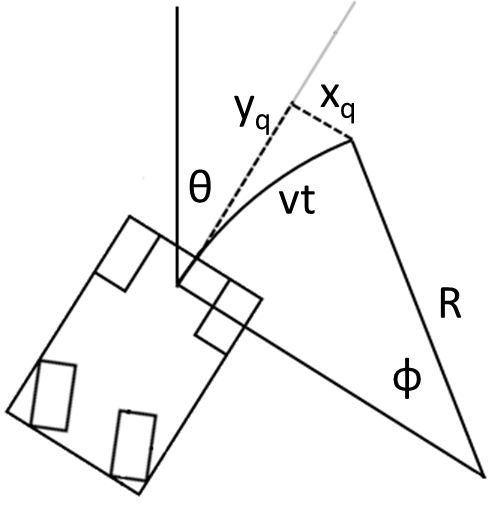
\includegraphics[width=0.5\textwidth]{4-DetailedDesign/quadbikeKinematics.png}
\centering
\caption{Quad bike kinematics} \figlabel{quadKinematics}
\end{figure} 
so the prediction equation for $\bar{\mu_t},\ g(u_t,\ \mu_{t-1})$ becomes:
\begin{align}
g(u_t, \mu_{t-1}) &=
\begin{bmatrix}
	x_G + y_q\sin\theta + x_q\cos\theta\\
    y_G + y_q\cos\theta + x_q\sin\theta\\
    \theta + \phi
\end{bmatrix},\\
G = \frac{\partial g_i}{\partial x_j} &=
\begin{bmatrix}
    1	&	0	&	y_qcos\theta - x_qsin\theta\\
    0	&	1	&	-y_qsin\theta - x_qcos\theta\\
    0	&	0	&	1
\end{bmatrix}
\end{align}
This needs to be recalculated at each prediction step as well as it's Jacobin, $G$. The process noise for the prediction, $\delta_t$, is represented by a Gaussian distribution with covariance $R$.
\begin{align}
R =
\begin{bmatrix}
    \sigma_x^2	&	0	&	0\\
    0	&	\sigma_y^2	&	0\\
    0	&	0	&	\sigma_\theta^2
\end{bmatrix}
=
\begin{bmatrix}
    (0.025 \times V\Delta t)^2	&	0	&	0\\
    0	&	(0.025 \times V\Delta t)^2	&	0\\
    0	&	0	&	(0.97 \times V\Delta t)^2
\end{bmatrix}
\end{align}
Where $\sigma_x, \sigma_y, \textrm{and } \sigma_\theta$ are based on the accuracy of readings given by the velocity and steer angle sensors on the quad bike. Testing (see \secref{testingwheelencoder}) showed the error in distance, ($\sigma_x, \sigma_y$), to consistently vary within 0.5 m for every 20 m travelled, or 0.025 m/m. Since the heading is calculated based on the distance travelled and the turn angle, the error is also dependent on these factors. The steering motor is accurate to 1 degree of the true value due to initialisation and the error is maximum when at full lock due to the trigonometric function present in the turn angle equation below. The difference in turn angle at full lock when a 1 degree error is present is then:
\begin{align}
&\Delta\phi = \frac{V\Delta t}{\frac{L}{\tan\ 24}} - \frac{V\Delta t}{\frac{L}{tan\ 23}} = \frac{V\Delta t}{2.87} - \frac{V\Delta t}{3.02} = 0.017V\Delta t = 0.97\ \degree/m
\end{align}
Positional and angular data from the GPS and angular data from the IMU are observed. In the case of the GPS, the EKF inputs are the observation matrix and its Jacobian:
\begin{align}
h(\mu_t) = 
\begin{bmatrix}
    x_{gps}\\
    y_{gps}\\
    \theta_{gps}
\end{bmatrix}\\
H = \frac{\partial h_i}{\partial x_j} &= 
\begin{bmatrix}
    1	&	0	&	0\\
    0	&	1	&	0\\
    0	&	0	&	1
\end{bmatrix}
\end{align}
And an observation error modelled by a Gaussian distribution with covariance matrix $Q$:
\begin{align}
Q = 
\begin{bmatrix}
    \sigma_x^2	&	0	&	0\\
    0	&	\sigma_y^2	&	0\\
    0	&	0	&	\sigma_\theta^2
\end{bmatrix}
=
\begin{bmatrix}
    0.4^2	&	0	&	0\\
    0	&	0.4^2	&	0\\
    0	&	0	&	20^2
\end{bmatrix}
\end{align}
As the GPS drifts when stationary, positional data from this sensor is only used when the platform is at cruising speed, or when travelling in a forwards direction at 5 km/hr. Experimental data showed the GPS to be accurate within 0.4 m at this speed, and therefore the calculated heading accurate within ~20 degrees when measuring between subsequent points. This on its own is not accurate enough as it exceeds the desired positional accuracy.  

Therefore, the IMU is also used to correct the heading. As only one element of the state vector is being updated the matrix math is set up slightly differently. Experimental data shows the IMU has an error of approximately 2 degrees per 360 degrees travelled.
\begin{align}
h(\mu_t) = \mu_t &= 
\begin{bmatrix}
    \theta + \Delta \theta_{imu}
\end{bmatrix}\\
H = \frac{\partial h_i}{\partial x_j} &= 
\begin{bmatrix}
    0	&	0	&	1
\end{bmatrix}
\end{align}
And an observation error modeled by a Gaussian distribution with covariance matrix $Q$:
\begin{align}
Q = 
\begin{bmatrix}
    \sigma_\theta^2
\end{bmatrix}
=
\begin{bmatrix}
    (\frac{2}{360}\Delta \theta_{imu})^2
\end{bmatrix}
\end{align}
With the inputs calculated a new estimate covariance, $\Sigma_t$, and position estimate, $\mu_t$, is outputted to be used in the next iteration of the algorithm. 

\chapter{Arduino Code Chart}
\chaplabel{arduinoCodeChart}
\begin{figure}[ht]
\centering
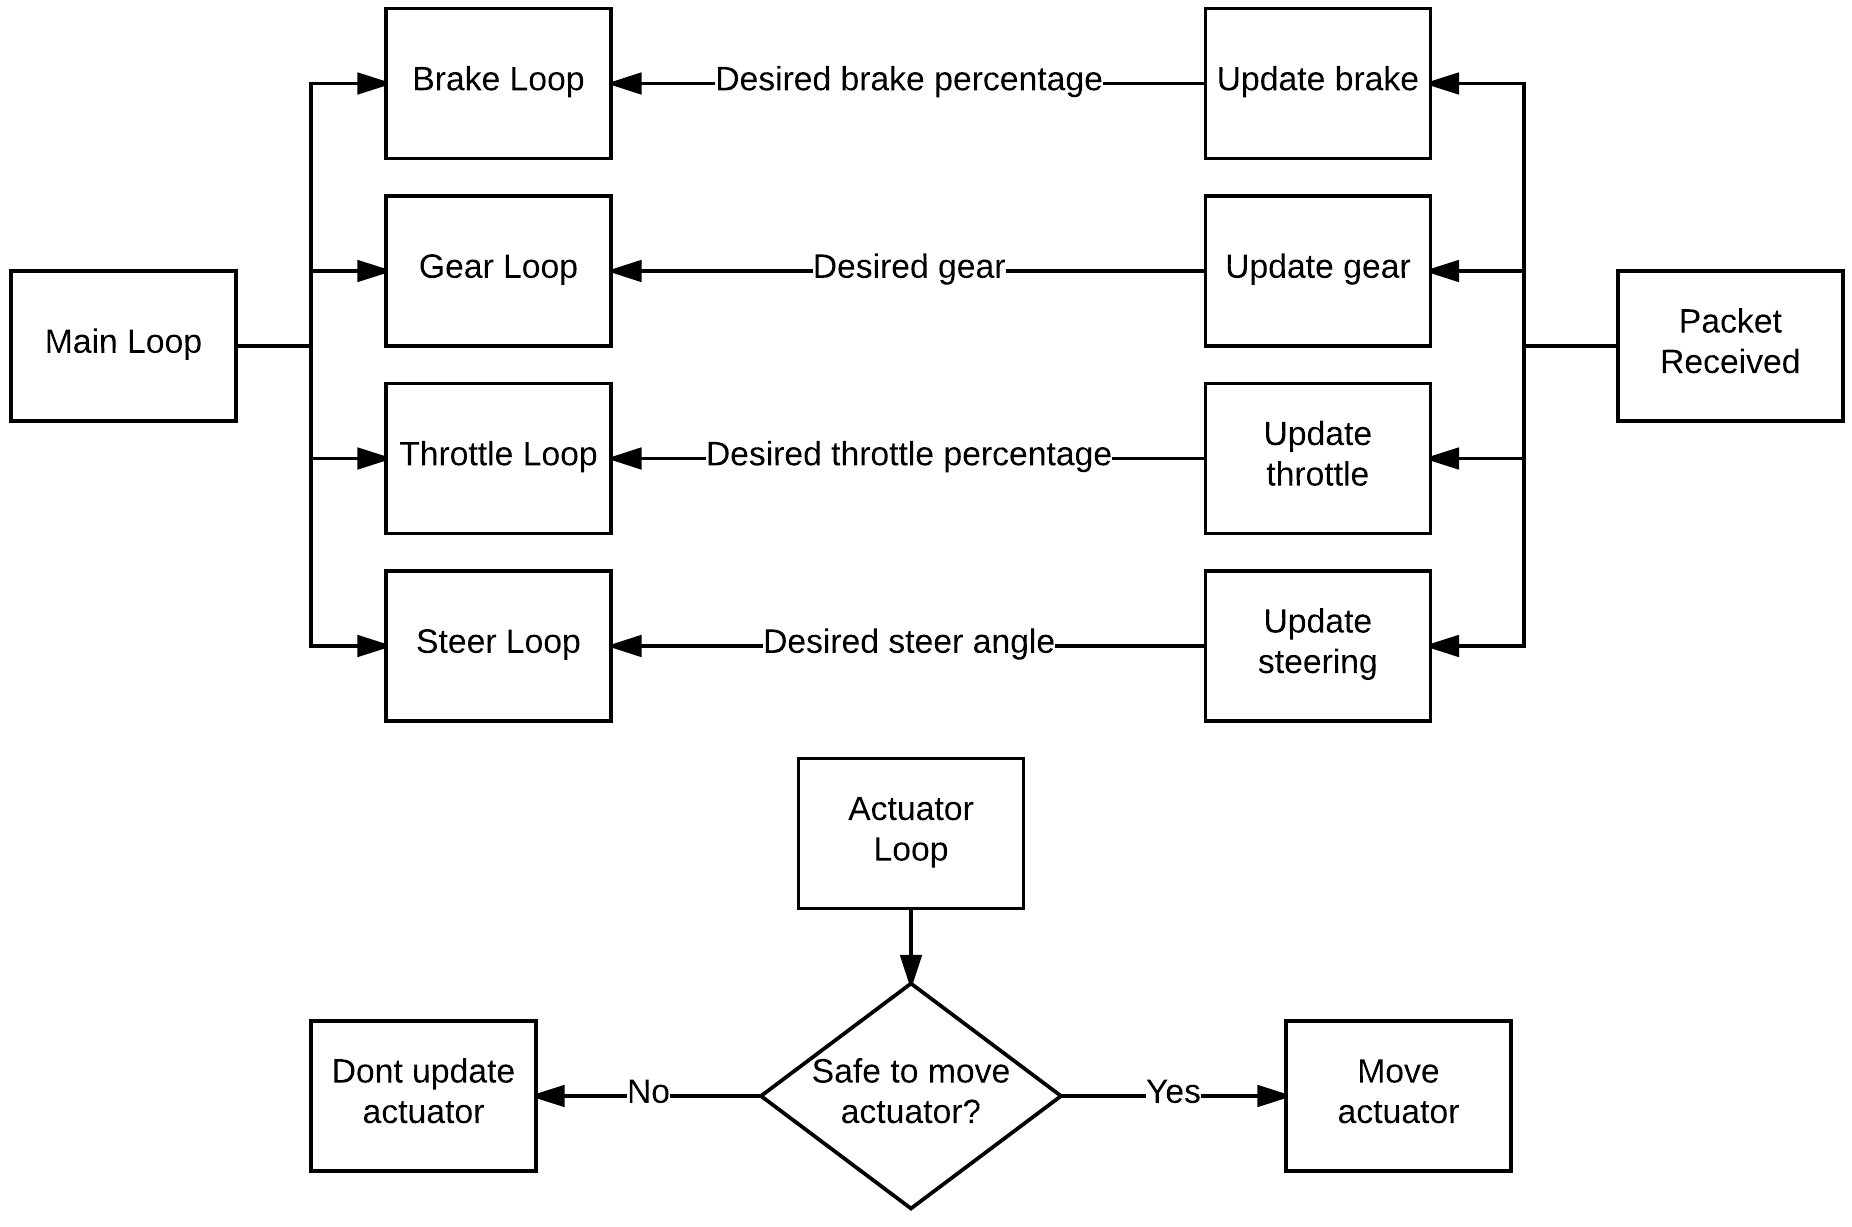
\includegraphics[]{8-Appendices/arduinoDiagram.png}
\end{figure}

\chapter{Sensor Mount Vibrations Analysis}
\chaplabel{sensorVibesApp}
While it is difficult to model the vibrational modes of a beam exactly, approximate analytical solutions for lower order modes may be obtained using classical methods. Two such methods are the Rayleigh and Dunkerly methods. The Rayleigh method considers the energy balance at the location of each beam mass element. A solution for the modes can be obtained based on knowledge of the static deflection. In general, the Rayleigh method provides an upper limit for the fundamental frequency. The Dunkerly method considers a force balance along the beam, which leads to the result that the overall modes are a superposition of the modes of the individual elements. The Dunkerly method generally provides a lower limit for the fundamental frequency.
\textcolor{red}{some references?}
Both methods were used to find the vibrational modes for three different configurations. The first configuration is a simple cantilever with self weight, the second is a massless cantilever with an end-loading, while the third is a cantilever with self-weight and an end loading.  \Tabref{theoreticalvibestable} shows the results for each of the different configurations and methods.

%\[
%Cross section: 35 x 70 mm    	Length: 1.5 m
%Density: 515 \frac{kg}{$m^3}   	Modulus of elasticity: 10.06 GPa 
%End load mass: 5 kg 			Beam mass = 1.8926 kg (calculated)

%\]

\begin{table} [ht]
\centering
\caption[Theoretical vibration results using Rayleigh and Dunkerly methods]{Theoretical vibration results using Rayleigh and Dunkerly methods for a 35 x 70 x 1500 mm beam in different configurations }
\tablabel{theoreticalvibestable}
\begin{tabular} {r c c}
\toprule
Configuration & f Dunkerly (Hz) & f Rayleigh (Hz)  \\ \midrule
Cantilever (1.9kg self weight) & 22.2097 & 34.0655  \\
Cantilever (massless, 5kg end load) & 6.7321 & 6.7321 \\
Cantilever (1.9kg self weight , 5kg end load) & 6.4427 & 6.8844 \\ \bottomrule
\end{tabular}
\end{table}

A cantilever beam of self weight was analysed in ANSYS. The transverse vertical fundamental frequency was found to be 27.707 HZ which lies between the frequency ranges found from using the Dunkerly and Rayleigh methods. This validates that the FEA model is working correctly and can be used to model the sensor mount accurately.

The modes for the sensor mount were found to be 17.89 Hz. The addition of the cross member supports add stiffness to the frame resulting in the increased frequency over a standard cantilever beam. The vertical supports act to reduce the length of the cantilever beam further increasing the fundamental frequency. The deflections caused to the frame due to the fundamental frequency was 32.805 mm as can be seen in \Figref{Finalframeansys2}. 

\begin{figure}[ht]
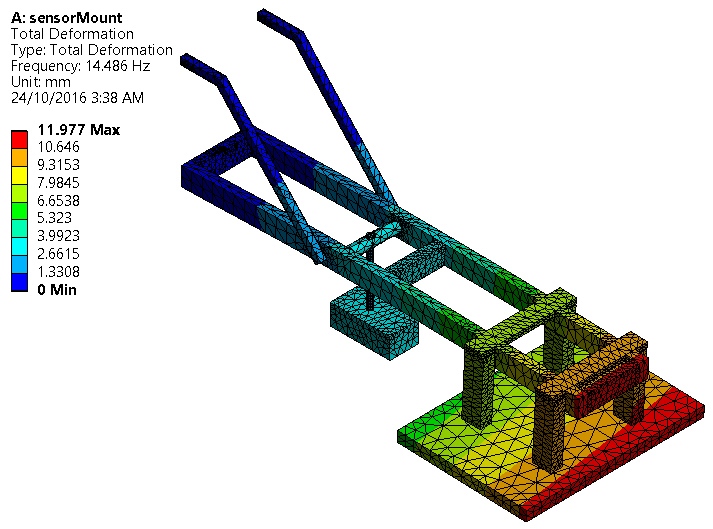
\includegraphics[width=0.7\textwidth]{4-DetailedDesign/vibrations.PNG}
\centering
\caption{Sensor mount vibrational analysis} \figlabel{Finalframeansys2}
\end{figure} 

The addition of the metal detector to the frame resulted in fundamental frequencies of 13.647, 14.573 and 31.913 Hz with a maximum deflection of 9.9417 mm. The addition of the weight of the metal detector acts to dampen the fundamental frequency as expected. This same damping can be seen from the theoretical results for the cantilever beam with the added end weight.

Variations in sensor arrangements that could be installed would result in different fundamental frequencies due to the changing damping effects. This can be accounted for by increasing of decreasing the length of the frame to change the fundamental frequency to one that is desired. The frame design can be tuned to a specific fundamental frequency through the alteration of its design and end weight.   


\chapter{Software Design Documents}
\chaplabel{designDocs}


\chapter{Communications Packet Formats}
\chaplabel{packets}

\begin{enumerate}
\item 
\textbf{Packet Identifier}\\
\textit{1 unsigned byte} \\
This will be a byte from the enumerator list included in the Packet.h file.
the value of this ID will indicate to the receiver what the packet data is. This could be a command, or an indicator of what the data type is and where it should go to. The 
\item
\textbf{Packet Length}\\
\textit{1 unsigned byte}\\
Indicates the length of the float array
				passed in this packet. Accepts values in the range 0 - 255. For packets carrying no data, this will be zero.
\item
\textbf{Packet Data}\\
\textit{Between 0 and 1024 bytes, in increments of 4, interpretable as IEEE 754 floats (4 bytes per float)}\\
An array of floats containing arbitrary data, length as specified. The way this data will be interpreted will be determined by the packet ID. This is detailed in the code documentation as to what data each packet ID is expected to carry. 
\end{enumerate}

A typical valid packet will be of the following format:\\

0x \textcolor{blue}{01} 52 \textcolor{blue}{01} 3F 8C CC CD \textcolor{blue}{17}\\

This format is explained in the \Tabref{packetBreakdown} below.

\nohyphens{	% Stop hyphenation in table
\begin{longtable}{L{0.2\textwidth} L{0.25\textwidth} L{0.45\textwidth}}
\caption[Stakeholders]{Stakeholders of the project.}\tablabel{packetBreakdown}\\ \toprule
\textbf{Item} & \textbf{Hexadecimal} & \textbf{Description}\\ \midrule\endfirsthead 
\caption[]{Stakeholders of the project (continued).}\\ \toprule
\textbf{Members} & \textbf{Roles} & \textbf{Description}\\ \midrule\endhead

Peter Dawson & Project Manager, Document Manager & The project manager is responsible for the overall management of the project. Their tasks involve communicating with the supervisor, group members, project sponsor and other external parties. Additionally, they are responsible for assignment of tasks and chairing of meetings. The document manager is responsible for document collation and data backup. \\ \midrule

Jonathan Targett & Technical Manager & The technical manager’s responsibility is the overall management of the technical aspects of the project. The technical aspects may include procurement mechanical resources, electronic resources and other materials for the project.\\ \midrule

Rahul Kalampattel & Safety Manager & The safety manager is responsible for lloking after the safety aspects of the project. This includes conducting risk assessments, providing a safe operating procedure (SOP), overseeing the completion of such documents and liaising with the necessary third parties to provide relevant safety information.\\ \midrule

Racquel Punu & Secretary, Test Manager & The secretary is responsible for the administrative requirements of the project, including producing meeting minutes, and submission of documents through MyUni. The test manager is responsible for overall management of any testing conducted on systems and their components as required.\\ \midrule

Harrison Vince & Treasurer, Manufacturing Manager & The treasurer is responsible for managing finances within the project. The manufacturing manager is responsible for overseeing any manufacturing processes undertaken, and dealing with other design related issues.\\ \midrule

Dr Maziar Arjomandi & Project Supervisor & Supervises student members and guides them accordingly.\\ \midrule

DSTG & Project Partner and Sponsor & Supports the project and project members in providing expertise, loaning of equipment, and funding. A research agreement entitles the Project Partner to share in all knowledge gained over the course of the project.\\ \bottomrule

\end{longtable}}


%%%%%%%%%%%%%%%%%%%%%%%%%%%%%%%%%%%%%%%%%%%%%%%%%%%%%%%%%%%%%%%%%%%%
%%%%%%%%%%%%%%%%%%%%%%%%%%%%%%%%%%
%TEST PROCEDURES

\chapter{Testing Procedures}
\chaplabel{testProcedureApp}
%%%%%%%%%%%%%%%%%%%%%%%%%%%%
% Test cases enum for quad bike
\newcounter{qb}[section]
\renewcommand*{\theqb}{%
%   \ifnum\value{req}<1000 0\fi%
%   \ifnum\value{req}<100 0\fi%
  \ifnum\value{qb}<1 0 \fi%
  \arabic{qb}% 
}
\newenvironment{qb}[1][]{\refstepcounter{qb}\par\medskip\indent{}
   \textbf{TC 1.\theqb:#1} \rmfamily}{\bigskip}
%%%%%%%%%%%%%%%%%%%%%%%%%%%%%

%%%%%%%%%%%%%%%%%%%%%%%%%%%%
% Test cases enum for GPR
\newcounter{gpr}[section]
\renewcommand*{\thegpr}{%
%   \ifnum\value{req}<1000 0\fi%
%   \ifnum\value{req}<100 0\fi%
  \ifnum\value{gpr}<1 0 \fi%
  \arabic{gpr}% 
}
\newenvironment{gpr}[1][]{\refstepcounter{gpr}\par\medskip\indent{}
   \textbf{TC 2.\thegpr:#1} \rmfamily}{\bigskip}
%%%%%%%%%%%%%%%%%%%%%%%%%%%%%

%%%%%%%%%%%%%%%%%%%%%%%%%%%%
% Test cases enum for GPR
\newcounter{mds}[section]
\renewcommand*{\themds}{%
%   \ifnum\value{req}<1000 0\fi%
%   \ifnum\value{req}<100 0\fi%
  \ifnum\value{mds}<1 0 \fi%
  \arabic{mds}% 
}
\newenvironment{mds}[1][]{\refstepcounter{mds}\par\medskip\indent{}
   \textbf{TC 3.\themds:#1} \rmfamily}{\bigskip}
%%%%%%%%%%%%%%%%%%%%%%%%%%%%%

\section{Goals}
The development of a functioning platform with landmine detection using ground penetrating radar (GPR) and metal detector panel. Platform tests includes subsystem breakdowns and independent system testing to identify and confirm their functionality. These subsystems include steering, braking, throttle control, gear selection, wheel encoder, and navigation (GPS). Sensor tests identify how the signals detected by the GPR and metal detector panel vary under differing conditions, and how this impacts the ability to identify a landmine effectively. This plan outlines the testing approach, sequence and specific instructions required to meet the project objectives. 

% \section{References}
% Documentation relevant to each system are referenced accordingly to provide additional information regarding the performed tests.

% \subsection{Platform}
% \begin{itemize}
% \item Quad bike safety operating procedure and risk assessments
% \item SmartMotor
% \item Quad bike navigation software
% \item Quad bike electronics manual 

% \end{itemize}

% \subsection{Ground penetrating radar}

% \begin{itemize}
% \item Safety operating procedure and risk assessment for the GPR
% \item Reference to GPR theory and literature
% \item SIRO-Pulse II factsheet
% \item SIRO-Pulse II operating manual
% \item Laptop operational sheet 
% \end{itemize}


% \subsection{Metal detector panel}
% \begin{itemize}
% \item Safe Operating Procedure and risk assessment (3187) for the metal detector panel
% \item Relevant metal detector theory as outlined in literature review
% \item Bruschini, C. (2002) A multidisciplinary analysis of frequency domain metal detectors for humanitarian demining, PhD thesis, Vrije Universiteit Brussel, Brussels.
% \item Minelab metal detector specifications (yet to be obtained)

% \end{itemize}

\section{Test plan}
A systems breakdown for the whole project in respects to testing is required. The quad bike and sensory systems are required to be tested independently in order to determine their individual operating states before fusing them together. The quad bike will require subsystem tests leading up to full system automation tests wile the sensory systems will require data collection and analysis in order to produce the required metrics for the software decision making processes. In order to complete this, each system requires a test plan to be created. The test plan highlights the testing objective for each system and their corresponding subsystems as well as the required outcomes. These outcomes are essential to the goals and objectives of the project as they allow for the project as a whole to advance forwards.

\subsection{Testing objectives}
In order for a successful test plan to be created, objectives are required. These are chosen as the building blocks that when accumulated together create the final product. The testing objectives are broken down into the quad bike subsystem, the metal detector and the GPR. The testing objectives allow for the test cases to be generated with a measurable outcome.

\subsubsection{Quad bike}
The quad bike systems will be broken down into individual mechatronic subsystems for testing to identify if any components need replacing and the characteristics of the subsystem. The tests will encompass the steering, braking, throttle, gear selecting, wheel encoder, GPS, and engine systems to ensure correct operation.

\medskip\noindent
Initial testing will be conducted with the quad bike on its stand for its ease to work on, manoeuvre as required and for the added safety as the wheels are not in contact with the ground. Independent tests on each subsystem will be conducted to determine their operational status, how best to control them, and how to control them autonomously. Once these are all completed for each subsystem, Whole system testing will commence whereby the quad bike is allowed to traverse a designated area under remote control. Autonomous testing will be conducted once all systems are able to be controlled and shut down remotely.

\medskip\noindent
The tests will be divided into subsystems of the quad bike to ensure that individual subsystems are functioning. This includes overall system start and shut-down, electronic components, steering, braking, throttle and actuating systems. The tests will be conducted at an overall system level in order to:
%\begin{enumerate}
%\item Identify and confirm function of electronic components
%%%%%%%%%%%%%%%%%%%%%%%%%%%%
% TEST CASES
%%%%%%%%%%%%%%%%%%%%%%%%%%%%
%\subsubsection{Quad bike}

% Use this counter for quad bike
\begin{qb}
\textbf{Identify and confirm function of electronic components}\\
\textbf{Objective:} Test that all quad bike electronics are functioning. Identify, replace, and record any broken devices and upgrade any obsolete systems. Determine, label, and record all subsystem electronic pins for future reference in the event that they are removed and replaced. Correctly working electronics will allow for more reliable operation of the platform.

\end{qb}

%\item Confirm the startup and shutdown procedure 
\begin{qb}
\textbf{Confirm the startup and shutdown procedure}\\
\textbf{Objective:} Test that the Quad bike is able to be started and that the engine runs smoothly and continuously before turning it off. All emergency stops, both physical and electronic will be tested to ensure that they turn off the quad bike as required. This is needed for the safety of people in close proximity to the platform in the event of a malfunction.  

\end{qb}

\begin{qb}
\textbf{Determine functionality of the steering actuation}\\
\textbf{Objective:} Test steering actuation and control. Determine if stepper motor, or limiting switches are adequate. Test controllability and speed of wheel movement as well as maximum turn angles in each direction. Accurate knowledge of the steering motion will allow for more accurate navigation and control. Knowing the exact steering angles and if the motions are repeatable is important for the navigational software as it will have effects on the position. 

\end{qb}

\begin{qb}
\textbf{Determine functionality of the brake actuation}\\
\textbf{Objective:} Test brake actuation to ensure that it is functioning correctly. Determine if a faster brake actuator is needed to meet platform stopping requirements. Conduct stationary tests before commencing dynamic tests up to operational speeds. The brake is important to the control and navigation of the platform. Braking authority will allow for tighter manoeuvres and bring the platform to a stop before rolling over a detected landmine. 

\end{qb}

\begin{qb}
\textbf{Determine functionality of the throttle actuation}\\
\textbf{Objective:} Test throttle actuation to ensure that the actuator is working correctly. First test in neutral and increase engine throttle remotely, then conduct straight line tests at slow speeds. The required throttle ranges for forwards and reverse motion will be required. Accurate throttle positioning will ensure the quad bike is able to operate at a constant and repeatable speed. Control over the throttle will allow for the platform to come to a stop even without brakes.

\end{qb}

\begin{qb}
\textbf{Determine functionality of the gear actuation}\\
\textbf{Objective:} Test gear actuator and that the  correct gear is being selected. Find the limiting range of motion defined by the linear potentiometers so that the gear selecting mechanism is not damaged by the actuator. This will allow for forwards and reverse motion to be achievable as defined in the platform and navigation requirements.  

\end{qb}


\begin{qb}
\textbf{Determine functionality and accuracy of the wheel encoder}\\
\textbf{Objective:} Check that wheel encoder is working correctly and that it is accurate and corresponds with electronic output on quad bike display unit. Check that the speed and subsequent distances travelled calculated through the wheel encoder are accurate and repeatable. The accuracy of the wheel encoder has large effects on the of the navigation and positioning systems. Knowing the exact speed and distances travelled are important to the completion of the project as they have effects on the automation. 

\end{qb}
%\item Determine functionality of the steering actuation
%\item Determine functionality of the brake actuation
%\item Determine functionality of the throttle actuation
%\item Determine functionality of the gear actuation
%\item Identify and evaluate GPS output units
%\item Determine functionality and accuracy of the wheel encoder
%\end{enumerate}


\medskip\noindent 
Testing of the system as a whole is required to carried out in order to determine how each subsystem interacts with each other. This also incorporates the testing of the navigation and communication software for the remote control functionality of the quad bike. The tests conducted will be used to:

%\begin{enumerate}
%\item Determine required throttle percentage for ground motion
\begin{qb}
\textbf{Determine required throttle percentages for ground motion and operational speed}\\
\textbf{Objective:} Find the throttle percentages required to get the quad bike moving forwards and maintain a constant speed of 5 km/h. Gradually increase the throttle by 5\% increments until it starts moving forwards. Increase throttle until the quad bike is maintaining a constant speed of 5 km/h forwards. These will be the throttle ranges for motion. This is important to the navigation and potion software as accurate knowledge of the control systems for the quad bike is necessary for automation. 

\end{qb}

\begin{qb}
\textbf{Determine braking delay from activation to actual brake intensity being experienced}\\
\textbf{Objective:} Determine the brake delay in actuation from the brake command being sent, to the quad bike experiencing actual braking force. Determine the use case for the brakes for the navigation software and the times when it will be required.

\end{qb}

%\item Determine turning radius
\begin{qb}
\textbf{Determine braking distance}\\
\textbf{Objectives:} The quad bike will travel forwards for a measured 3.5 m marked by a flag, then apply the brakes. The final distance will be marked and the distance between the brake marker and the final position of the quad bike will be the braking distance. There is an aim to reduce the effective braking distance as the quad bike is required to stop within 60 cm to avoid detonation a detected landmine. 

\end{qb}
%\item Test remote control functions 
\begin{qb}
\textbf{Test remote control functions}\\
\textbf{Objectives:}The ability to control the platform remotely will lead to easy implementation of automation and navigation software. This will require command inputs from a remote tablet and the quad bike outputs will be measured. Each subsystems will be tested individually to ensure their correct functionality before live tests on the ground. Tests with the virtual platform will also be completed to check that the correct commands are being sent to the quad bike.  
\end{qb}
%\end{enumerate}

\medskip\noindent 
Testing of the navigation software is the final step. This incorporates all the information and refinements discovered throughout the previous tests conducted. The navigation tests will be conducted in order to:

% \begin{enumerate}
% \item Determine accuracy of positioning devices, required for orientation and distance travelled
\begin{qb}
\textbf{Determine accuracy of positioning devices, required for orientation and distance travelled}\\
\textbf{Objectives:} For the GPS, a known path will be traversed and logged data compared with real coordinate data. A stationary test should also take place. From this, confirmation of accuracy and error data should be found. The IMU should be tested on both the quad bike while running and a non-vibrating surface. Time dependant drift and cumulative error should be measured.
\end{qb}

% \item Determine accuracy of virtual platform motions compared to real life motions of the quad bike
\begin{qb}
\textbf{Determine accuracy of positioning system}\\
\textbf{Objectives:} In both the virtual platform and actual positioning devices, the results of the Kalman Filter should be analysed. Information of interest includes accuracy, relative drift speed, and distance/time to stability.
\end{qb}


% \item Check the angle of turns and path following abilities of the platform when compared to desired performance. A straight line test will be conducted in order to sync up the Virtual display to the real world motion. Once the distance and motion is similar angled turns will be conducted. these will first be simple turns with gradual angle increases until complex angle turns are required. A 90 degree turn will be executed to check the accuracy and navigation performance before full automation tests can be performed. 
\begin{qb}
\textbf{Check the angle of turns and path following abilities of the platform when compared to desired performance.}\\
\textbf{Objectives:} A straight line test will be conducted in order to sync up the Virtual display to the real world motion. Once the distance and motion is similar angled turns will be conducted. These will first be simple turns with gradual angle increases until complex angle turns are required. A 90 degree turn will be executed to check the accuracy and navigation performance.

\end{qb}

% \end{enumerate}

\subsubsection{Ground penetrating radar}

The ground penetrating radar’s characteristics and data generated will verify  and compare the signals produced from changes in frequency, material type, soil properties and depth. The tests will be conducted at an overall system level in order to:
% \begin{enumerate}
% \item Identify the GPR frequency used to produce the optimum strength and quality of signal 
\begin{gpr}
\textbf{Identify GPR frequency to be used}\\
\textbf{Objectives:} Confirm which of the three GPR frequency heads to use between 800 MHz, 1.4 GHz and 2 GHz. The frequency is required to be selected to optimise the penetration depth and resolution of signals received by the GPR. 
\end{gpr}
% \item Identify the signals generated by different types of materials
\begin{gpr}
\textbf{Identify the signals generated by different types of materials}\\
\textbf{Objectives:} Confirm that different materials affect the amplitude of signals reflected by the object to the GPR. Identify the signatures of the replica (dummy) landmines and clutter objects. This is to be able to extract necessary features from the GPR data to use in designed algorithms. 
\end{gpr}

% \item Identify the depth limit at which the GPR can detect an object
\begin{gpr}
\textbf{Test objects at different depths}\\
\textbf{Objectives:} Confirm the sensitivity of signals received based on target depth. This identifies how large or small the signals are for three different increasing depths to be able to calculate the output metrics as accurate as possible. 
\end{gpr}
% \item Identify how object data signals change with soil types
\begin{gpr}
\textbf{Identify how object data signals change with soil types}\\
\textbf{Objectives:} Confirm that for each different types of soil,  the signal strength (resolution) reflected changes and penetration ability may be hindered. The effect of certain types of soil hinders the ability to extract the features accurately. 
\end{gpr}

\begin{gpr}
\textbf{Confirms functionality of GPR signal processing algorithm}\\
\textbf{Objectives:} The data from the GPR is processed using the designed algorithm and stored in the database to define the output metrics such as feature width and feature depth. The test will enable further development of the algorithms designed. 
\end{gpr}

% \item Identify how environmental conditions affect signals 
% \end{enumerate}

\medskip\noindent
The tests will be completed outdoors with the GPR head and scanned over the objects. Manual scanning will be completed to ensure consistent speed over the objects. Further details of the test environment will be completed in the 

\medskip\noindent
Input parameters will be identified for each test case to provide consistency in data produced. These parameters include, and are not limited to: the initial settings as set by the SIROPULSE II program as defined in the user manual, different types of objects, type of soil and depths targets are buried.

\subsubsection{Metal detector panel}
The data generated by the metal detector in different tests will be verified against results described in literature. These results will also be used to test the algorithms designed to extract phase angle and magnitude of the target. The tests that will be conducted aim to:
% \begin{enumerate}
% \item Identify the differences between signals for ferrous and non-ferrous objects
\begin{mds}
\textbf{Identify the differences between signals for ferrous and non-ferrous objects}\\
\textbf{Objective:} Confirm that both ferromagnetic and non-ferromagnetic produce different phase plots. These phase plots will provide more information to identify which materials have similar signatures to landmines. 

\end{mds}

\begin{mds}
\textbf{Identify the frequency to be used}\\
\textbf{Objective:} Confirm which frequency to use out of the four provided by the metal detector. Certain frequencies produce a higher voltage magnitude for different types of targets.  

\end{mds}

% \item Identify the effect of target depth on detection 
\begin{mds}
\textbf{Identify the effect of target depth on detection}\\
\textbf{Objective:} Confirm that different depths corresponds to a change in magnitude of the voltage flux detected. Change in magnitude will assist in identification of the target object. 

\end{mds}
% \item Identify how signals change with soil types
\begin{mds}
\textbf{Identify how signals change with soil types}\\
\textbf{Objective:} Observe the effect of the soil on the magnitude and phase plot of the signals. This helps to improve the algorithm for background signal removal.  

\end{mds}
% \item Identify how environmental conditions affect signals 
% \item Confirm software program is working
\begin{mds}
\textbf{Confirms functionality of metal detector signal processing algorithm}\\
\textbf{Objective:} The data from the metal detector is processed using the designed algorithm. This will enable confirmation of the phase angle and magnitude and provide useful information for the database to be developed. Testing will enable improvement of the algorithm. 

\end{mds}
% \end{enumerate}

\medskip\noindent
Testing will be completed using a trolley, which allows the sensor mount to be placed on top and attached with the metal detector and pushed over the area at a constant speed. These tests will be completed outdoors as to simulate the real environment for landmine detection with the quad bike. 

\medskip\noindent
Input parameters will be identified for each test case to provide consistency in data produced and will be noted in the test procedure document for each test. 

\subsection{Fault reporting and data recording}
Test results will be saved in an appropriate data format and noted in the test procedure documents. Any faults or failures of the tests will be included in the test procedure document as additional comments. 

\subsection{Resource requirements}
% \begin{table}[ht]
% \centering
% \caption{Resource requirements for each subsystem}
% \label{resource}
% \begin{tabular}{llcll}
% System & Hardware & Software & Documents & Personnel\\
% Quad bike & & & & \\

% Ground penetrating radar & & & & \\
% Metal detector & & & & \\
% \end{tabular}
% \end{table}
\subsubsection{Quad bike resources}
\begin{itemize}
\item Quad bike
\item Quad bike stand
\item Arduino
\item Power supply or battery
\item Safety barrier such as bunting
\item Desktop pc with installed programs
\end{itemize} 

\subsubsection{GPR resources}
\begin{itemize}
\item GPR box containing all accessories, such as head, batteries, USB cable, optical cables etc. 
\item Laptop computer with SIROPULSE II program installed
\item Replica landmines
\item Clutter objects

\end{itemize} 

\subsubsection{Metal detector resources}
\begin{itemize}
\item AMDS metal detector
\item Metal detector control box
\item Power supply with 0.5A current and 12 V. 
\item Laptop computer with DataSpleen installed
\item Replica landmines
\item Clutter objects

\end{itemize} 

\subsection{Test environment}
\subsubsection{Quad bike}
The quad bike platform will be tested indoors in a laboratory with adequate ventilation. The quad bike will be placed on a wheeled stand to keep it stationary. 

If performing tests outdoors and on the ground, the quad bike will follow correct procedures as outlined in the safety operating procedure (SOP) document. 

\subsubsection{Sensor suite}
The GPR and metal detector will be used to scan a test area with objects buried in a grid. The target objects used are anti-tank, high metal and low metal content anti-personnel mines. The landmines are buried at 2.5 cm, 7.5 cm and 15 cm depths,  respectively. Clutter objects will be buried in a similar grid structure at 7.5 cm or 15 cm depth.

\subsection{Test responsibilities}
The people responsible for the tests are the project safety officer, the engineer and the test manager. The project safety officer approves and inducts the relevant persons conducting the tests. The engineer will supervise how the tests are completed and the test manager completes the tests as outlined in the test procedures.  

\section{Test procedures}
Every test case listed for each system and their relevant procedures are outlined in a separate testing procedures document.

%%%%%%%%%%%%%%%%%%%%%%%%%%%%%%%%%%%%%%%%%%%%%%%%%%%%%%%%%%%%%%%% 

\chapter{Gear Actuator Truth Table}

A risk assessment of the gear actuation system revealed that there was a high risk of significant damage being caused to components on the quad bike in the event that the actuator was allowed to extend beyond operational limits. These limits could not be firmly restricted with mechanical guards, and the existing system allowed for limits to be set in software by interpreting the position of the gear actuator by reading the positions of two linear potentiometers. 

Due to the high consequence of failure identified in the risk assessment, a state system was determined to be required to mitigate this risk. Under this scheme, each cycle of the code loop would update the control signals sent to the gear actuator based on the desired position and the current position as described by the potentiometers. This system is very robust against programmer error, as there is only a single position in the code where the input to the actuator is permitted to be changed. It also ensures that the actuator is continually checked to ensure that it is not accidentally left engaged without checking for over extension.

The truth table presented below details the actions that this state based system should take, based on all possible permutations of the inputs. Development of a truth table permits fast development and debugging of any issues, and was a crucial component in mitigating the risk of operating the gear actuator.


%\textcolor{red}{Add description of the gear actuator truth table}
\chaplabel{gearTable}
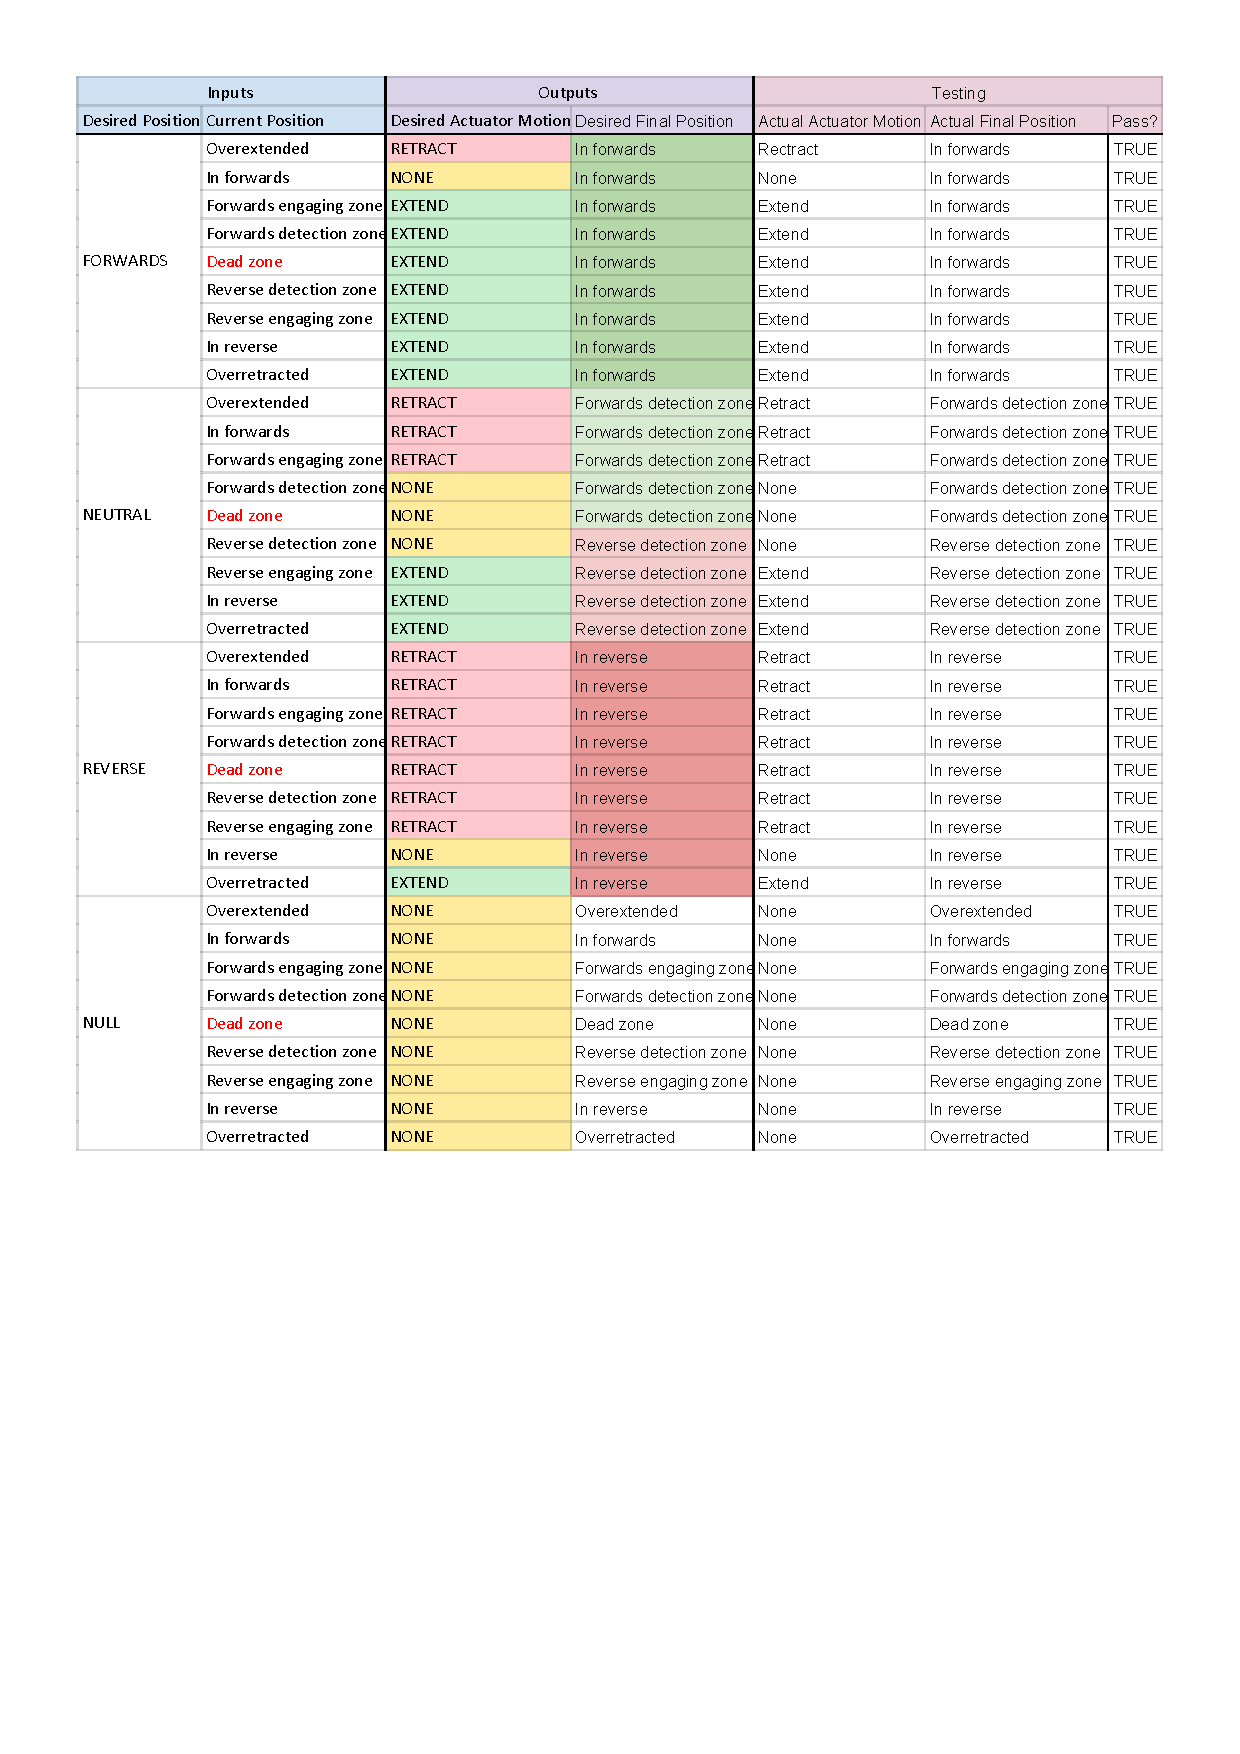
\includepdf[pages={1-}]{8-Appendices/gearTruthTable.pdf}



\chapter{Work Breakdown Structure}
\chaplabel{WBS}
The work breakdown structure shows how the technical workload of the project has been broken down into different  subsystems, and who has been assigned responsibility for managing each task. 

{\setstretch{1.15}
\begin{enumerate}
\item \textbf{Platform}\\
The platform subsystem comprises of the vehicle used to mount the sensor payload, the hardware required for automation and the physical landmine marking system. This subsystem is linked to the subsystems 3 (sensor mounting structure) and 4 (platform automation software).
	\begin{enumerate}[label*=\arabic*.]
	\item Benchmarking and literature review of platform (Harrison, Rahul)
    \item Develop specifications (Harrison, Peter)
    \item Concept designs and evaluation (Harrison, Peter)
	\item Platform evaluation and testing
    	\begin{enumerate}[label*=\arabic*.]
		\item Brake actuation (Harrison, Peter)
        \item Steering actuation (Harrison, Peter)
        \item Gears actuation (Harrison, Peter)
        \item Throttle actuation (Harrison, Peter)
        \item Platform testing (All)
        \end{enumerate}
    \item Physical landmine marking
    	\begin{enumerate}[label*=\arabic*.]
		\item Benchmarking and literature review (Jono, Racquel, Rahul)
        \item Concept designs and evaluation (Jono, Racquel, Rahul)
        \item Detailed design (Jono, Racquel, Rahul)
        \item Manufacture (Jono, Racquel, Rahul)
        \item Testing (All)
        \end{enumerate}
    \item Subsystem integration (All)
    \item Testing of integrated systems
    	\begin{enumerate}[label*=\arabic*.]
		\item Initial system testing (All)
        \item Field testing (All)
        \end{enumerate}
	\end{enumerate}
    
\item \textbf{Sensor system}\\
The sensor system includes the physical sensors that are used for landmine detection. This subsystem is linked to the subsystems 3 (sensor mounting structure) and 6 (landmine detection software).  
	\begin{enumerate}[label*=\arabic*.]
	\item Literature review on landmine detection methods
    	\begin{enumerate}[label*=\arabic*.]
        \item Metal detectors (Racquel)
        \item Ground penetrating radar (Jono)
        \item Other
		\end{enumerate}
    \item Evaluation of sensors provided by DSTG
	    \begin{enumerate}[label*=\arabic*.]
		\item Metal detector array (Jono, Racquel, Rahul)
        \item GPR (Jono, Racquel, Rahul)
        \end{enumerate}
    \item Sensor/platform integration (Harrison, Jono, Racquel)
    \item Process and interpret sensor output (Jono, Racquel)
    \item Testing (All)
    \end{enumerate}
    
\item \textbf{Sensor mounting structure}\\
The sensor mount subsystem allows the sensor payload to be mounted on the platform. This subsystem is linked to the subsystems 1 (platform) and 2 (sensor system).
	\begin{enumerate}[label*=\arabic*.]
	\item Benchmarking and literature review (Harrison, Rahul)
    \item Develop specifications (Harrison, Peter)
    \item Concept designs and evaluation (Harrison, Peter)
    \item Detailed design (Harrison, Peter)
    \item Manufacture (Harrison)
    \item Testing (Jono, Racquel, Rahul)
    \end{enumerate}
    
\item \textbf{Platform automation software}\\
The platform automation software allows the platform to operate without user input. This subsystem is linked to subsystems 1 (platform) and 5 (platform navigation software).
    \begin{enumerate}[label*=\arabic*.]
    \item Software requirements specifications (Jono)
    \item Software design document (Jono)
    \item Formulate development and testing methodology (Jono, Rahul)
    \item Primary development phase and evaluation (Jono)
    \item Secondary phase and evaluation (Jono, Rahul)
    \item Testing (Jono, Rahul)
    \end{enumerate}
    
\item \textbf{Platform navigation software}\\
The platform navigation software allows the autonomous platform to navigate a course without user input. This subsystem is linked to subsystems 4 (platform automation software) and 7 (application software). 
    \begin{enumerate}[label*=\arabic*.]
    \item Software requirements specifications (Harrison)
    \item Software design document (Harrison, Jono)
    \item Formulate development and testing methodology (Harrison, Jono)
    \item Primary development phase and evaluation (Harrison, Jono, Rahul)
    \item Secondary phase and evaluation (Jono)
    \item Testing (Jono, Racquel, Rahul)
    \end{enumerate}
    
\item \textbf{Landmine detection software}\\
The landmine detection software processes signals from the sensor system in order to detect landmines. This subsystem is related to subsystems 2 (sensor system) and 7 (application software).
    \begin{enumerate}[label*=\arabic*.]
    \item Software requirements specifications (Jono, Racquel)
    \item Software design document (Jono, Racquel)
    \item Formulate development and testing methodology (Jono, Racquel)
    \item Primary development phase and evaluation (Jono, Racquel, Rahul)
    \item Secondary phase and evaluation (Jono, Racquel, Rahul)
    \item Testing (Jono, Racquel, Rahul)
    \end{enumerate}
    
\item \textbf{Application software}\\
The application software allows an operator to remotely view the progress of the platform while it searches for landmines. This subsystem is linked to subsystems 5 (platform navigation software) and 6 (landmine detection software).
    \begin{enumerate}[label*=\arabic*.]
    \item Selection of control device (Jono)
    \item Software requirements specifications (Jono)
    \item Software design document (Jono)
    \item Formulate development and testing methodology (Jono)
    \item Primary development phase and evaluation (Jono)
    \item Secondary phase and evaluation (Jono)
    \item Testing (Jono, Racquel, Rahul)
    \end{enumerate}
\end{enumerate}}

\chapter{Gantt Chart}
\chaplabel{ganttChart}
The Gantt chart provides an overview of the timeline for the entire project. Major tasks are listed, as well as key milestones and deliverables. Tasks are assigned to team members, and progress on tasks is monitored at weekly meetings. Three Gantt charts are included in this appendix, the Gantt chart provided with the project charter, the Gantt chart provided with the preliminary report, and the most up-to-date version of the Gantt chart.
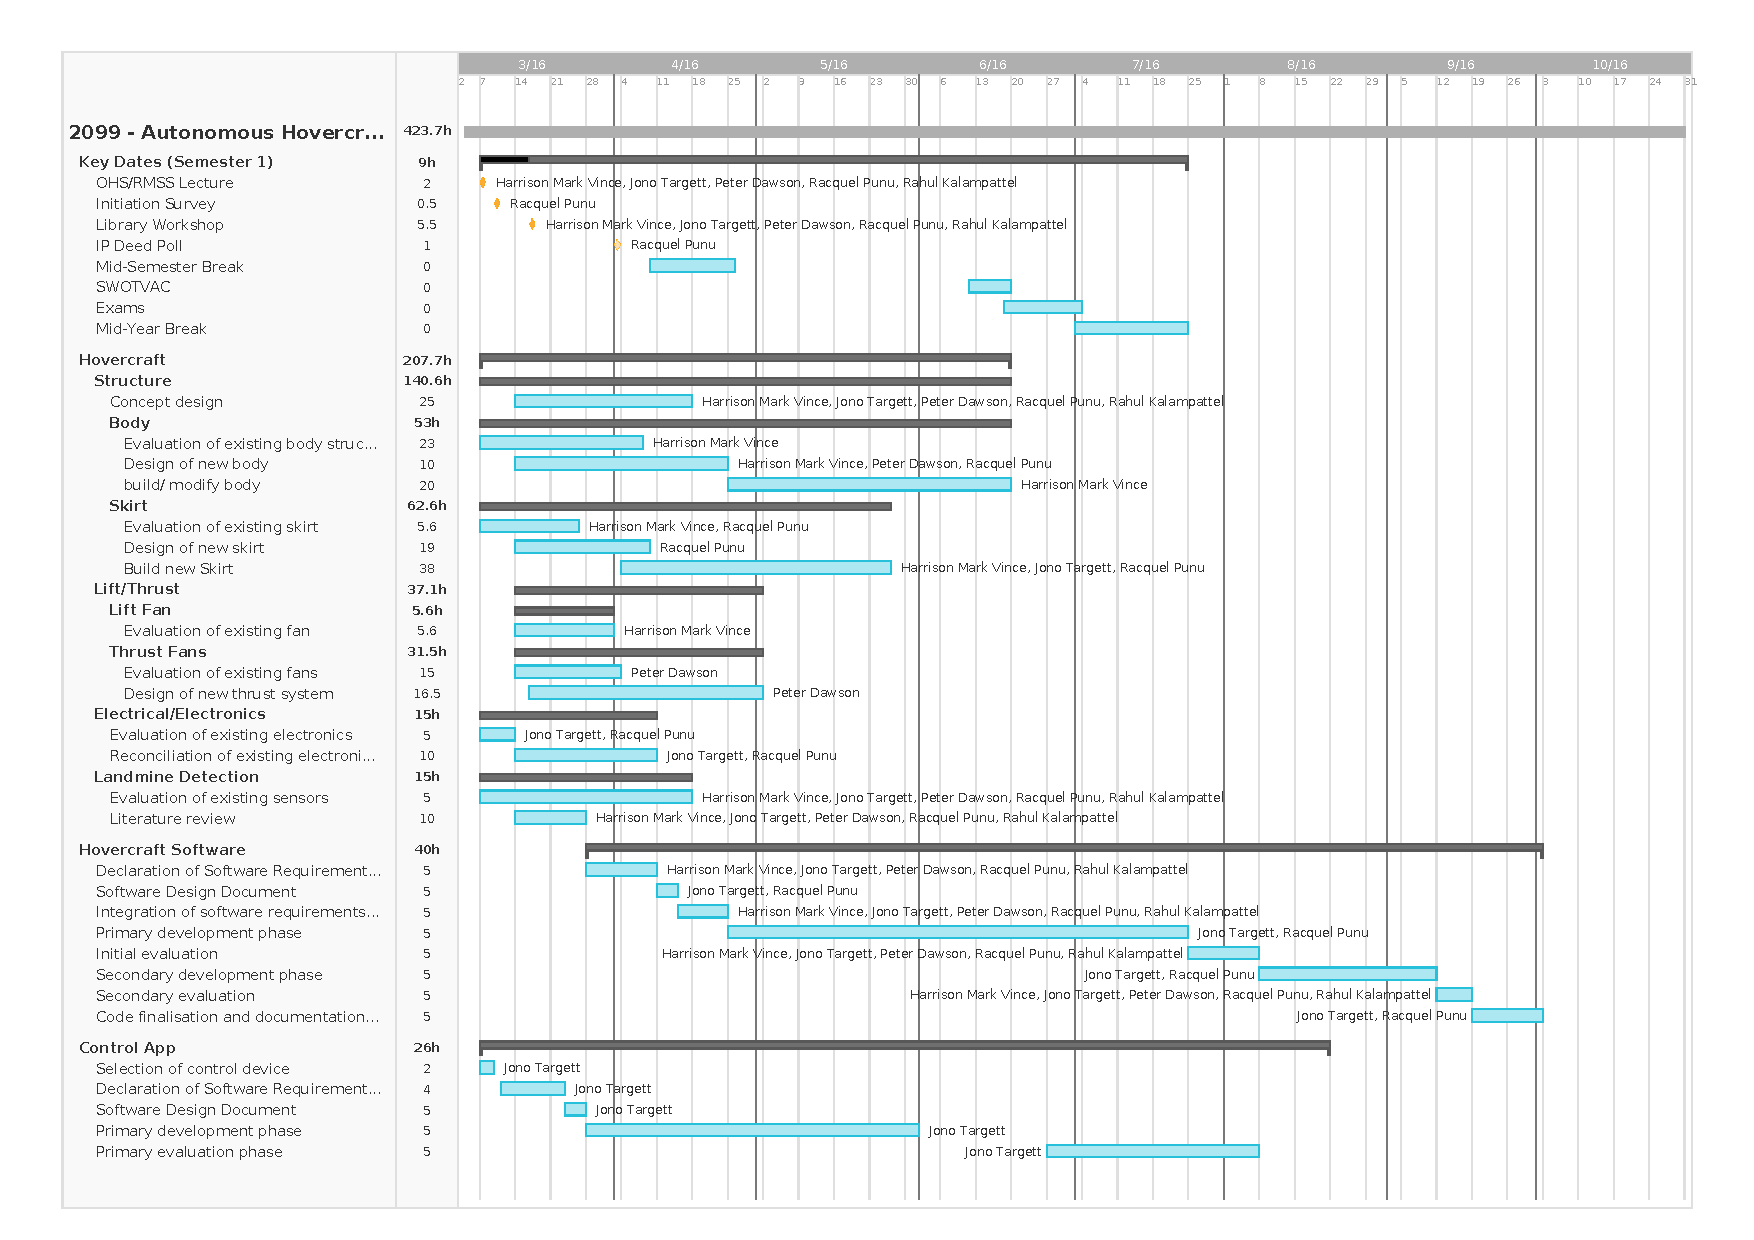
\includepdf[pages={1-},landscape]{8-Appendices/oldGantt.pdf}
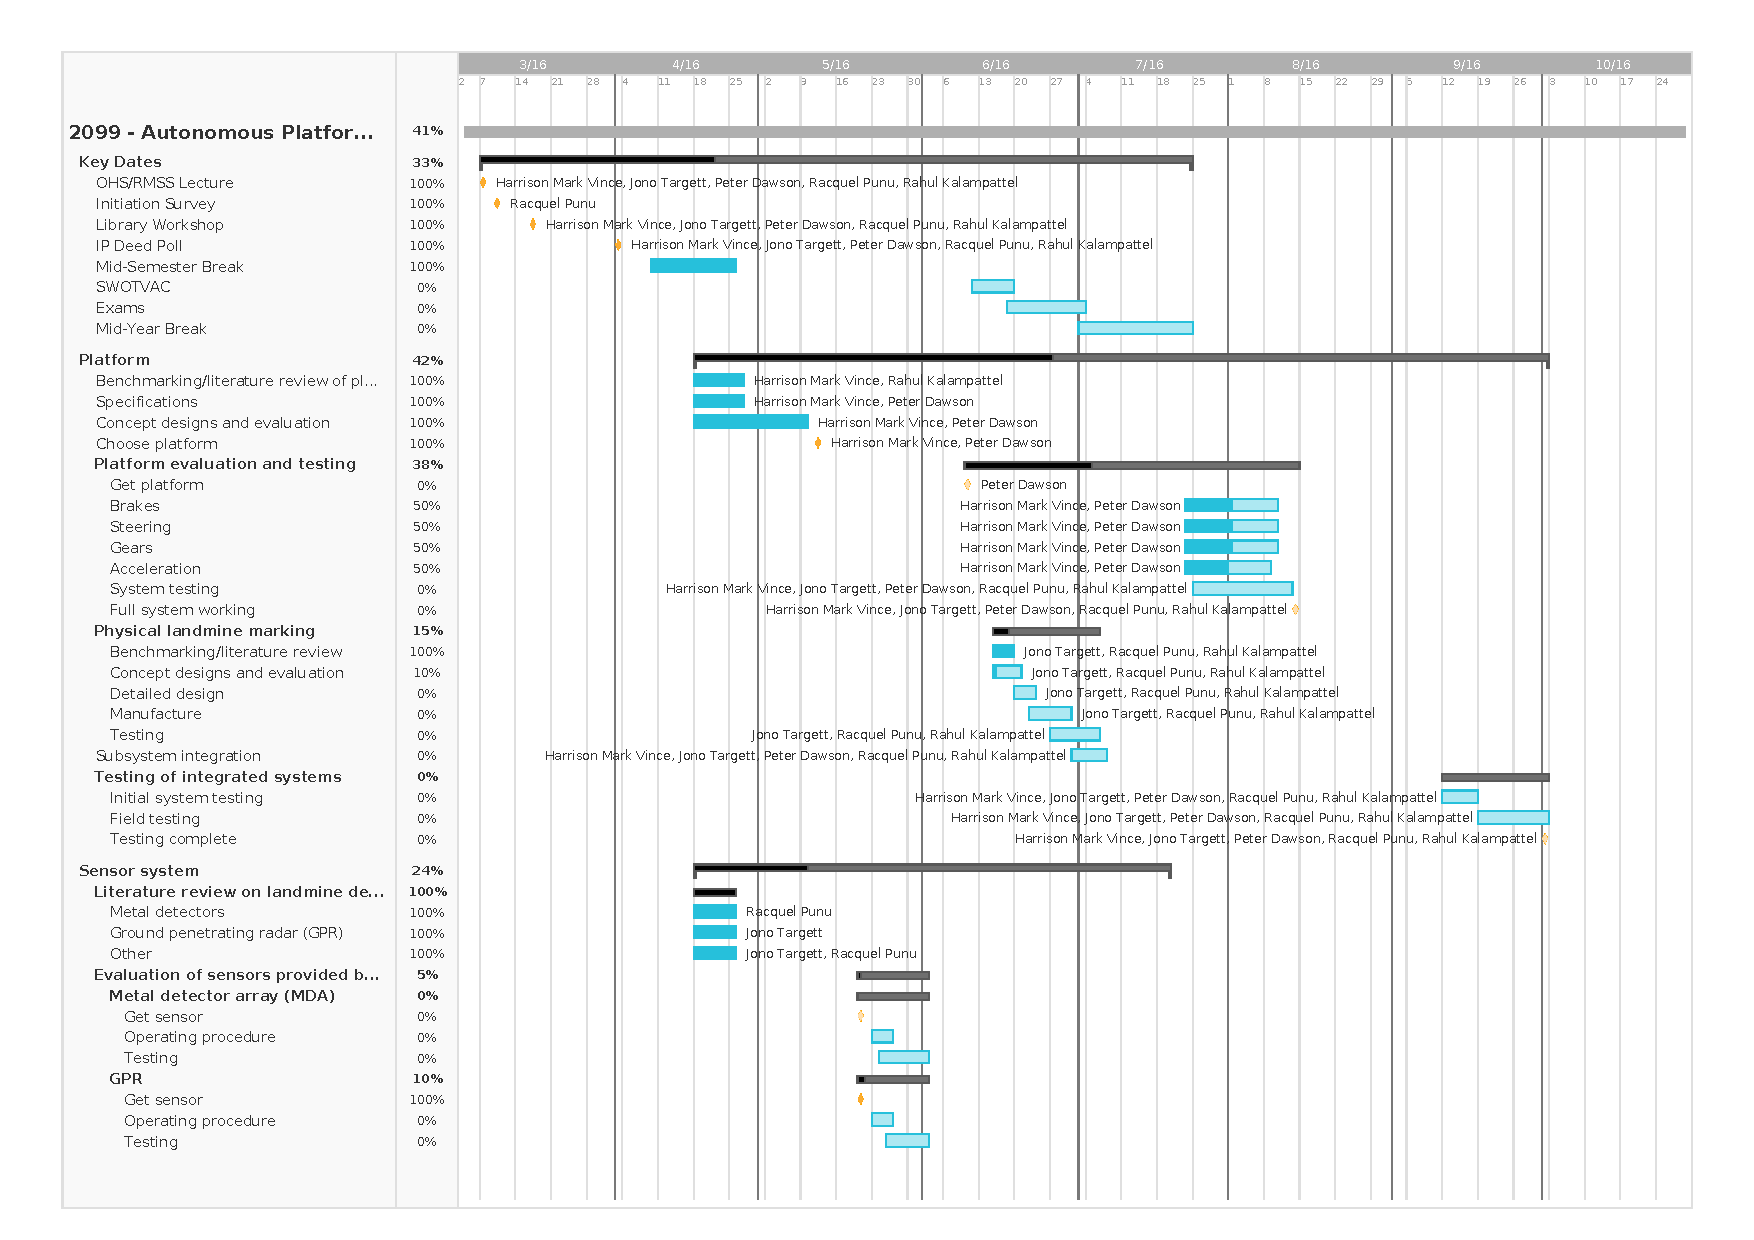
\includepdf[pages={1-},landscape]{8-Appendices/newGantt.pdf}
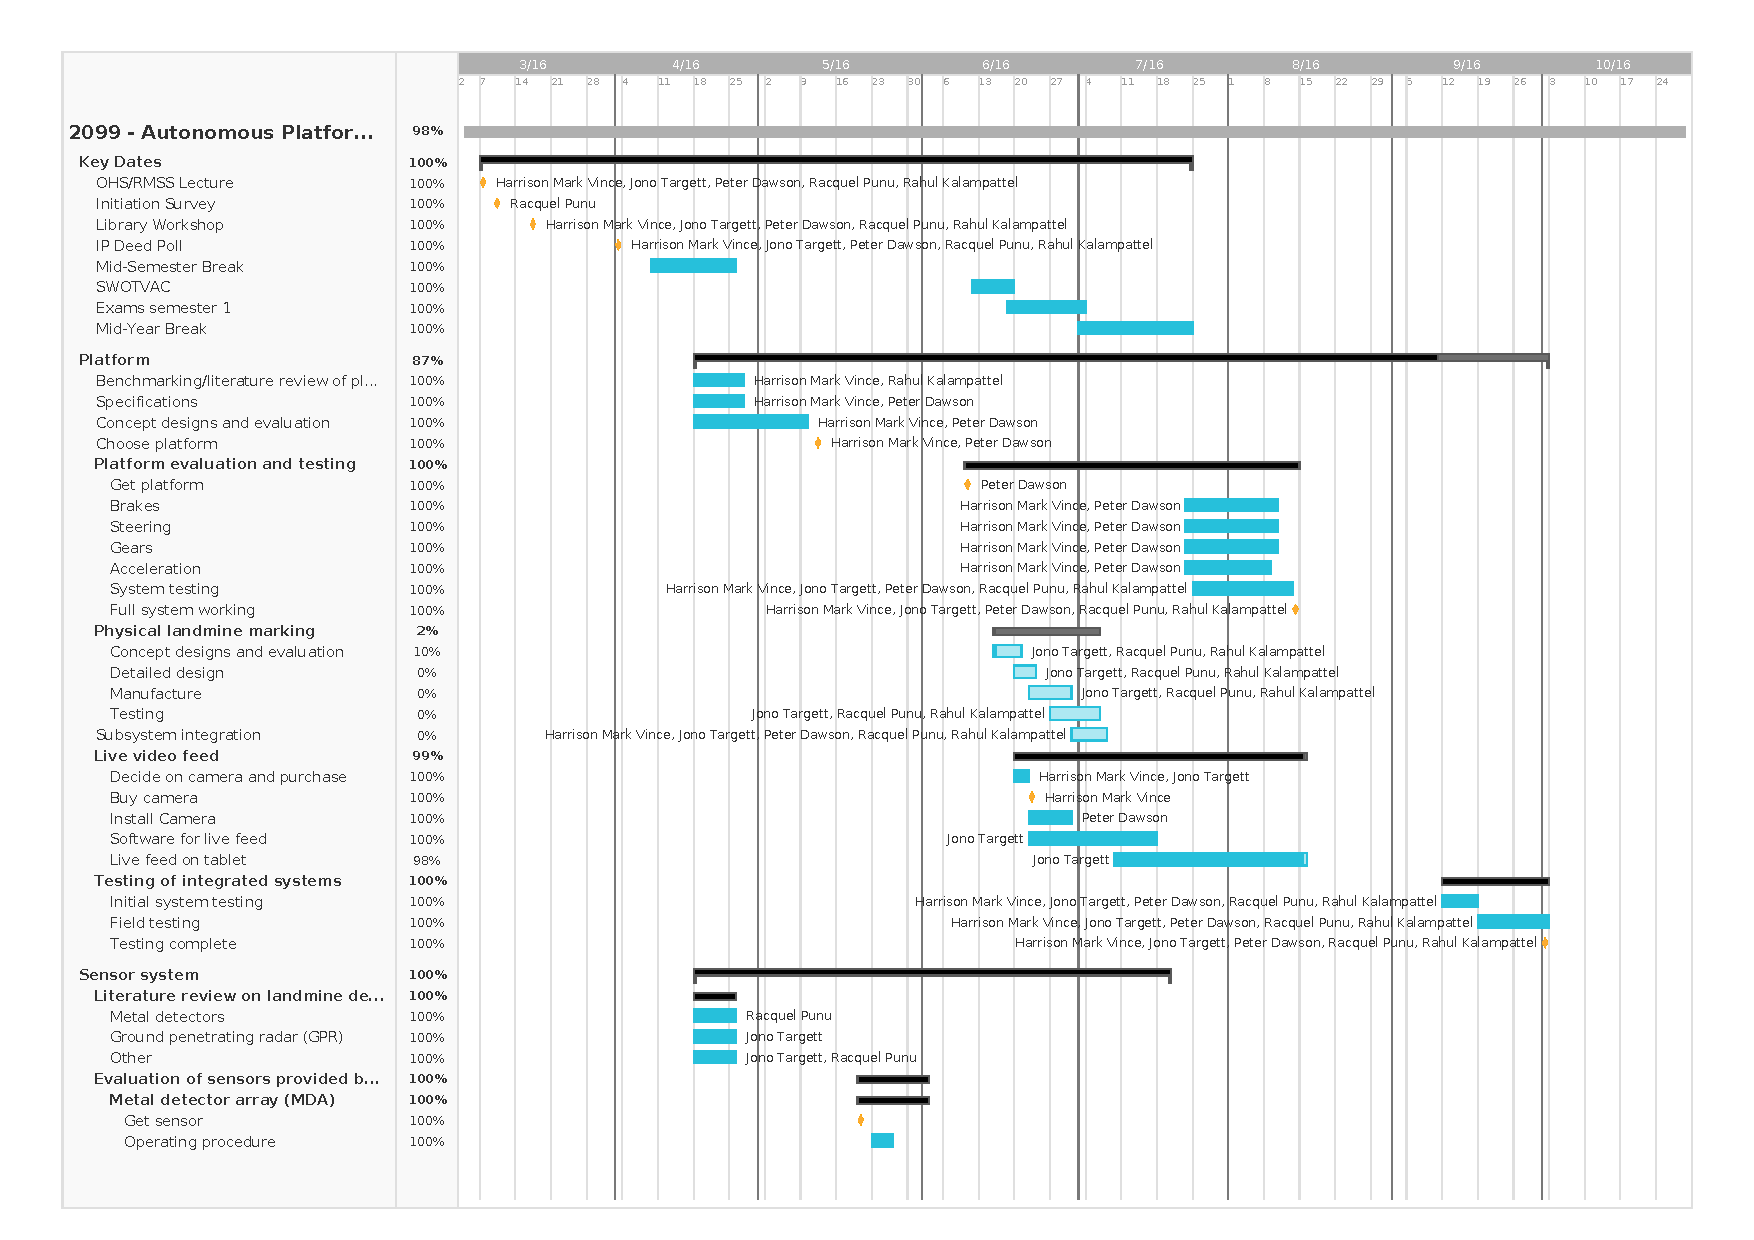
\includepdf[pages={1-},landscape]{8-Appendices/finalGantt.pdf}

\chapter{Safety Documents}
\chaplabel{riskAss}
As part of the formal risk management for the project, a risk assessment must be carried out using the RMSS system, and a safe operating  procedure (SOP) must be developed. Both of these items, as discussed in \secref{safety}, are attached on the following pages.
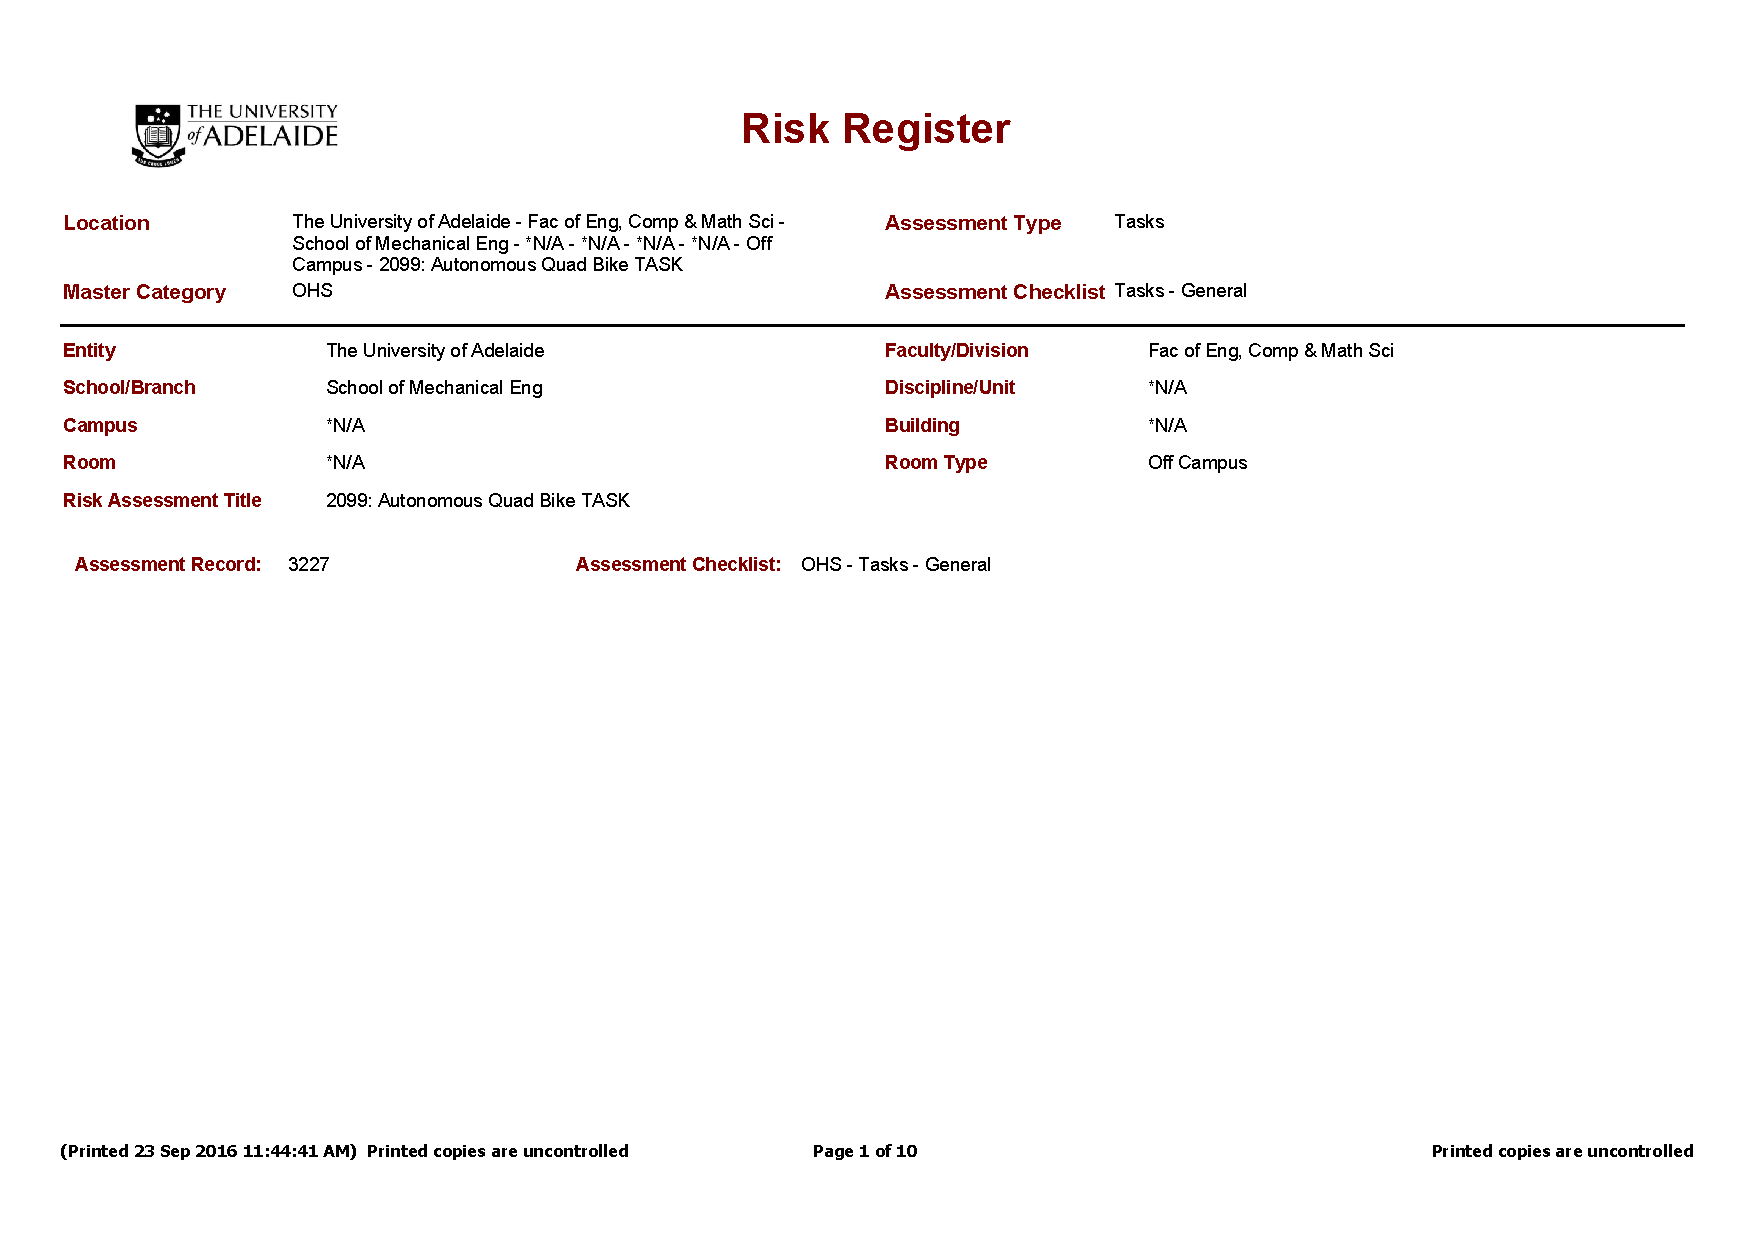
\includepdf[pages={1-},landscape]{8-Appendices/riskRegister.pdf}
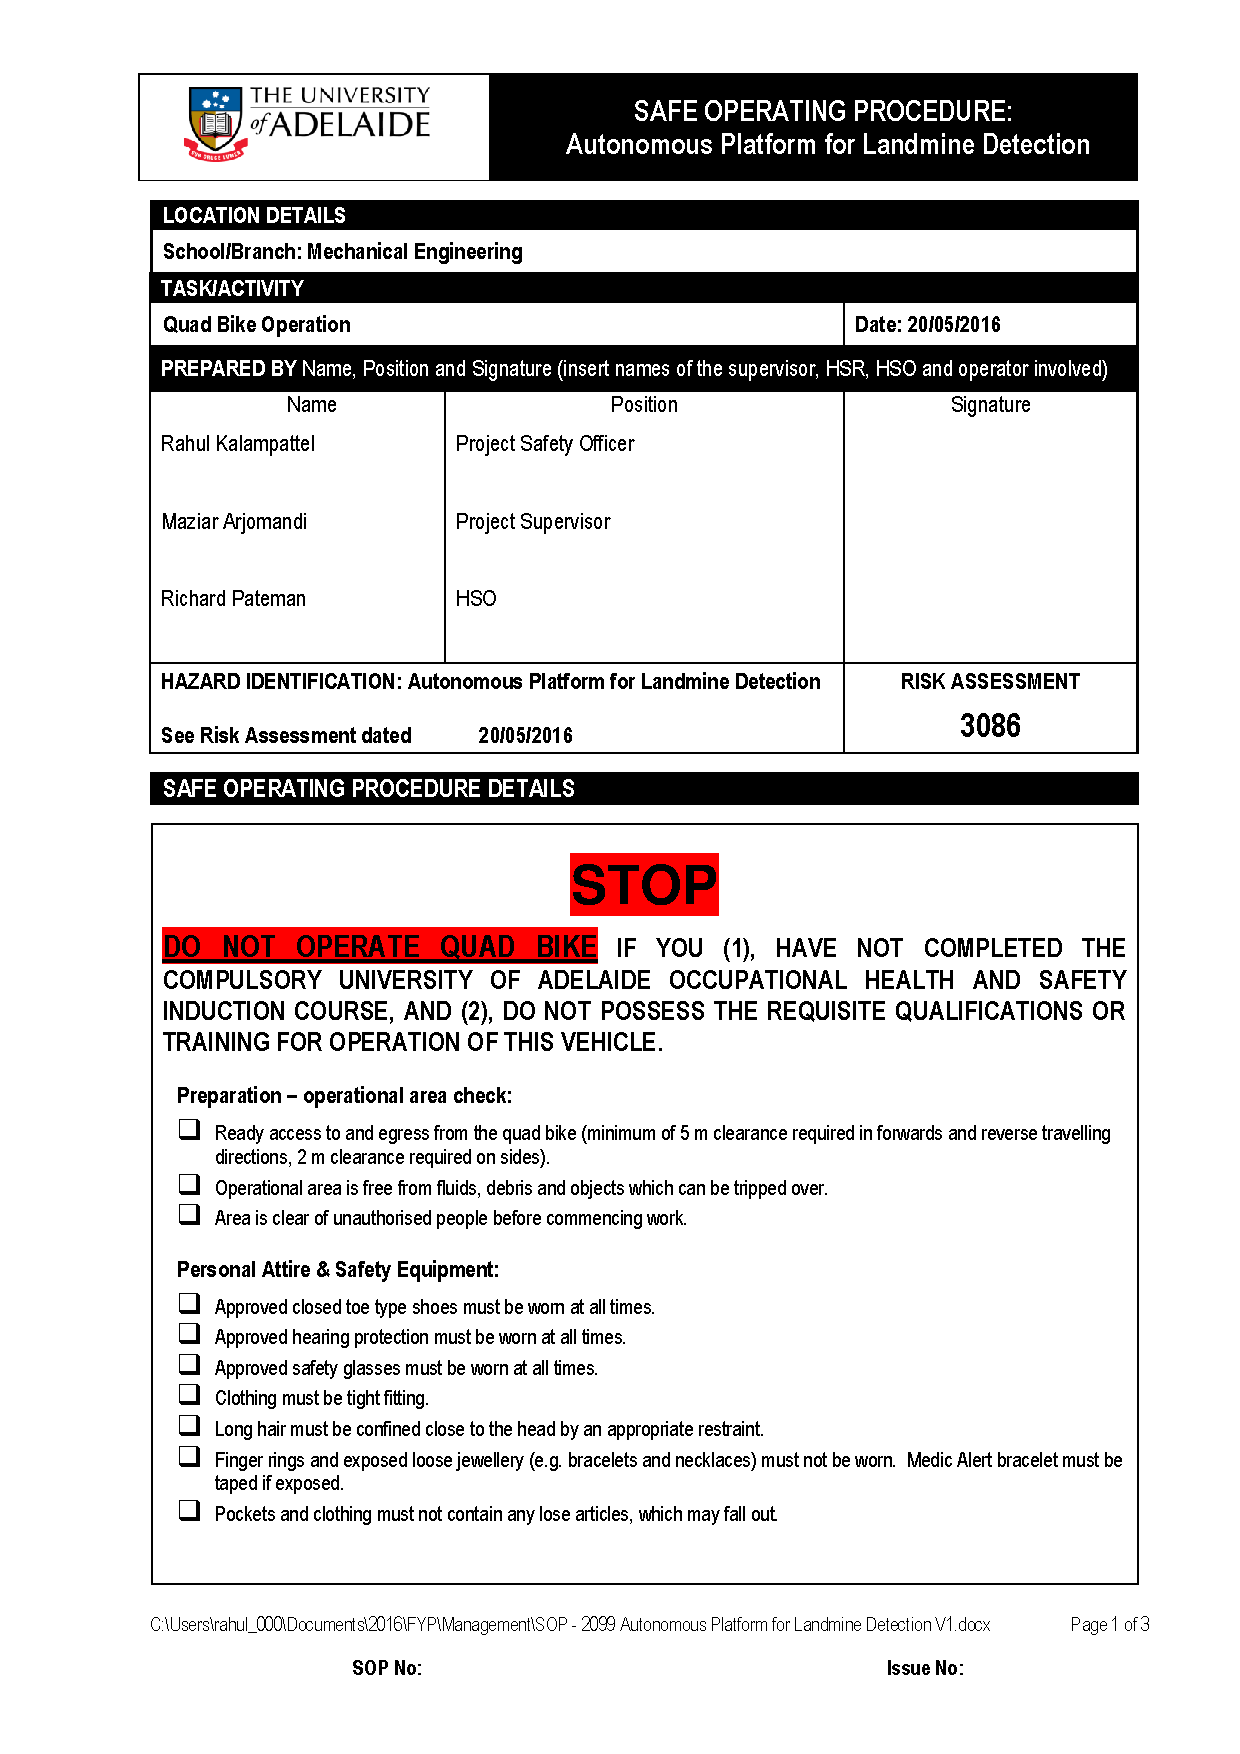
\includepdf[pages={1-}]{8-Appendices/SOP.pdf}

\chapter{Risks of Project Failure}
\chaplabel{riskFailureApp}
The risks to project failure are those events that may result in the project objectives not being completed. The risk level associated with an event is found by using the risk matrix, \Tabref{riskmatrix}.

\begin{table}[ht]
\caption{Risk matrix} \tablabel{riskmatrix}
\begin{tabular}{C{0.22\textwidth} C{0.22\textwidth} C{0.22\textwidth} C{0.22\textwidth}}
\toprule
\multicolumn{1}{c}{} & \multicolumn{3}{c}{\textbf{Impact}}\\ \cmidrule{2-4}
\textbf{Likelihood}&Minor&Moderate&Major\\ \midrule
Likely&\cellcolor{Yellow}Medium&\cellcolor{BurntOrange}High&\cellcolor{red}Extreme\\ 
Possible&\cellcolor{LimeGreen}Low&\cellcolor{Yellow}Medium&\cellcolor{BurntOrange} High\\ 
Unlikely&\cellcolor{OliveGreen}Negligible&\cellcolor{LimeGreen}Low&\cellcolor{Yellow}Medium\\ \bottomrule
\end{tabular}
\end{table}

\nohyphens{	% Stop hyphenation in table
\begin{longtable}{L{0.3\textwidth} L{0.1\textwidth} L{0.5\textwidth}}
\caption{Risk consequences, controls and recovery methods} \tablabel{risks}\\ \toprule
\textbf{Event} & \textbf{Risk} & \textbf{Consequences, controls and recovery}\\ \midrule\endfirsthead
\caption[]{Risk Consequences, Controls and Recovery Methods (continued)}\\ \toprule
\textbf{Event} & \textbf{Risk} & \textbf{Consequences, controls and recovery}\\ \midrule\endhead 

\multicolumn{1}{L{0.3\textwidth}}{\textbf{Existing platform unable to meet operational requirements}
The quad bike and associated hardware may not be sufficient to meet the performance specifications or achieve the project objectives} & \multicolumn{1}{L{0.1\textwidth}}{\cellcolor{Yellow}Medium} & \multicolumn{1}{L{0.5\textwidth}}{If the hardware on the quad bike does not function as well as required, it will be difficult to control the vehicle remotely, and even more difficult to automate. This will affect the entire system during the integrated testing stages of the project. In order to ensure that this does not become an issue later on, all aspects of quad bike will be tested and evaluated as soon as it is available. Necessary components will be serviced or replaced, and in the event that the extent of repairs is too large, sufficient funding is available to purchase a new platform.} \\ \midrule

\multicolumn{1}{L{0.3\textwidth}}{\textbf{Unable to successfully find targets}
The multi-sensor system may not be able to detect and confirm mines with a sufficient confidence level} & \multicolumn{1}{L{0.1\textwidth}}{\cellcolor{Yellow}Medium} & \multicolumn{1}{L{0.5\textwidth}}{Limited target detection and confirmation ability is likely to be due to difficulties encountered during signal processing and data fusion. This would mean the project goal could not be met. To reduce the likelihood of this occurring, a detailed plan has been devised for software development and testing. The multi-sensor system will only be tested once the performance of the individual sensor systems has been confirmed. In the event that the confidence level is still too low, simulated data can be used, allowing the testing of other related systems, such as the GPS logging system.} \\ \midrule

\multicolumn{1}{L{0.3\textwidth}}{\textbf{Automation and navigation cannot be achieved} Unable to operate the quad bike autonomously due to complexity, part failure or poor time management} & \multicolumn{1}{L{0.1\textwidth}}{\cellcolor{Yellow}Medium} & \multicolumn{1}{L{0.5\textwidth}}{Controlling the platform remotely is not anticipated to be a difficult task. Full automation of the system, to the level required for operation, carries increased risk due to complexity of the control software. To ensure that automation can be implemented successfully, control systems will be developed with a milestone based approach, whereby lower-level and simpler controls are implemented before more complex systems are commenced. Additionally, the software will be tested using a virtual platform.} \\ \midrule

\multicolumn{1}{L{0.3\textwidth}}{\textbf{Systems cannot be integrated}
Unable to use the sensor system in conjunction with the autonomous platform, either due to mounting issues or challenges with software} & \multicolumn{1}{L{0.1\textwidth}}{\cellcolor{LimeGreen}Low} & \multicolumn{1}{L{0.5\textwidth}}{An inability to integrate systems correctly will hinder testing, meaning the  project objective cannot be realised. Due to the small size and relatively insensitive nature of the sensors to disturbances, mounting will not be difficult. The high level software architecture will be developed in a way that allows for easy integration of systems. If any one of the component systems does not lend itself well to integration, its performance can be simulated.} \\ \midrule

\multicolumn{1}{L{0.3\textwidth}}{\textbf{Unable to find time to complete project}
Automating the platform, signal processing of sensor data and testing and integration prove too time consuming to manage with other commitments} & \multicolumn{1}{L{0.1\textwidth}}{\cellcolor{LimeGreen}Low} & \multicolumn{1}{L{0.5\textwidth}}{Not having enough sufficient time will mean that many of the objectives will not be completed. The likelihood of this occurring is reduced through effective project planning, i.e. the use of a Gantt chart, which enforces deadlines for individual tasks, hence reducing the possibility of failure. In the event that an individual is unable to complete a task, another member of the group will assist where possible.} \\ \midrule

\multicolumn{1}{L{0.3\textwidth}}{\textbf{Platform sustains damage or fails}
The quad bike is damaged during testing or undergoes structural, mechanical or electrical component failure} & \multicolumn{1}{L{0.1\textwidth}}{\cellcolor{LimeGreen}Low} & \multicolumn{1}{L{0.5\textwidth}}{If the quad bike is to crash, individual parts or the sensor payload may suffer damage. The quad bike could also injure an individual. The likelihood of this event is reduced by the fact that the platform will be travelling at low speeds, and the impact to the vehicle is reduced since it is designed for off-road use. Furthermore, an emergency stop switch and remote kill switch has been put in place as control measures. According to the SOP, inspections will be made before commencing operation, to make sure that the sensor payload is attached correctly. If the failure is of an electrical nature, directional control or autonomous capabilities may be lost. The likelihood of this occurring is small, however in the event that it does, parts can be replaced relatively easily and cheaply.} \\ \midrule

\multicolumn{1}{L{0.3\textwidth}}{\textbf{Unable to acquire parts in time}
Necessary parts for the control system, or replacement parts, are delayed} & \multicolumn{1}{L{0.1\textwidth}}{\cellcolor{LimeGreen}Low} & \multicolumn{1}{L{0.5\textwidth}}{If the delivery of parts takes too long, individual subsystems will be put behind schedule, as will the testing schedule of the entire platform. The likelihood of this is reduced through early research and selection of required parts, allowing for sufficient delivery time. In the event that parts do not arrive due to unforeseen circumstances, they can be substituted with available parts that may be of a similar specification.} \\ \bottomrule
\end{longtable}}
\newpage
\newgeometry{left=0.75in, right=0.75in, top=0.9in, bottom=0.8in}

%
%% 
%%% DON'T FORGET TO CHANGE THE GEOMETRY LATER
%%
%

\chapter{Budget Breakdown}
\chaplabel{budgetApp}
A detailed breakdown of the budget is provided in the following tables. \Tabref{expenditureCurrent} outlines total project expenditure while \Tabref{labourHours} provides a monthly breakdown of the hours spent on the project by each student and the associated costs. Salaries are calculated at the rate of \$26/hr, with other direct and indirect costs included. Direct costs incur an additional 30\% on top of salary for items such as superannuation, payroll tax, workcover, long service leave, etc. Indirect costs incur an additional 130\% on top of salary for items such as administration and tech support, infrastructure, rent, phone, internet, etc.

\nohyphens{	% Stop hyphenation in table
\begin{longtable}{L{0.20\textwidth} L{0.52\textwidth} L{0.18\textwidth}}
\caption{Project expenditure} \tablabel{expenditureCurrent}\\ \toprule
\textbf{Subsystem} & \textbf{Item} & \textbf{Cost (\$)} \\ \midrule\endfirsthead 
\caption[]{Current expenditure (continued)}\\ \toprule
\textbf{Subsystem} & \textbf{Item} & \textbf{Cost (\$)} \\ \midrule\endhead
\textbf{General} & Wireless-N network adapter &	20.00 \\
\textbf{electronics} &	Wired desktop (keyboard + mouse) &	19.00 \\
 &	Samsung 120GB SSD &	69.00 \\
 &	USB Extension &	29.00 \\
 &	3mm Heat Shrink &	1.18 \\
 &	Electrical terminal &	5.95 \\
 &	Electrical terminal &	5.95 \\
 &	Heatshrink &	2.90 \\
 &	Electrical terminals &	5.95 \\
 &	2 x Cable ties &	9.96 \\
 &	Header pin and male-female socket &	6.25 \\ \midrule
\textbf{Platform} & Battery SNS40ZLS &	109.47 \\
\textbf{replacement} &	4 x Housing 2.54mm 3 way &	1.56 \\
\textbf{parts} &	2 x Housing 2.54mm 4 way &	1.00 \\
 &	Header Pin 40 way &	0.64 \\
 &	POT LIN 16mm 5k &	1.86 \\
 &	14 x Contact for 4072-1x04h 10k Reel &	3.08 \\
 &	4 x Micro SPDT 37mm lever &	15.09 \\
 &	3 x Cable Rainbow Ribbon &	10.64 \\
 &	GST from 20/07 &	3.51 \\
 &	10A Fuses &	3.50 \\
 &	Battery SNS40ZLS &	109.47 \\
 &	Linear position resistive sensor 5kohm &	91.16 \\
 &	nuts and bolts &	3.54 \\
 &	2 x electrical terminal &	17.85 \\
 &	Electrical cable 3 core &	5.80 \\ \midrule
\textbf{Platform} & Bunting & 65.00 \\
\textbf{testing} & Cable ties for bunting & 29.98 \\
 &	Sunscreen & 17.99 \\
 &	Warning flag & 6.67 \\ \midrule
\textbf{Platform} & Arduino Mega &	91.35 \\
\textbf{upgrade} & Proto shield extension Arduino &	7.77 \\
\textbf{parts} & Arduino proto extension kit &	19.91 \\
 & Remote control battery - 9.6V NiCd &	39.95 \\
 & Switch mode dc/dc converter &	683.48 \\
 & TTL to USB serial converter cable &	32.71 \\
 & GST from 08/08.2016 &	81.74 \\
 & Nuts bolts &	0.33 \\
 & I2C logic converter &	6.50 \\
 & 10DOF MPU6050 &	29.67 \\
 & 10 x Ultrasonic sensor &	19.00 \\
 & 3xArduino Mega &	50.40 \\
 & USB AM BM Cable &	3.06 \\
 & Transducer &	314.85 \\
 & MAX232N + adaptor board &	16.80 \\
 & GPS &	25.00 \\
 & Nuts and bolts for transducer &	18.8 \\
 & Emergency stops  &	177.47 \\
 & Emergency stop wiring &	71.94 \\
 & Petrol for quad bike	 & 13.79 \\
 & Camera WIFI IP 720p &	169.00 \\ \midrule
\textbf{Sensor} &  Structural pine 70x35 6m	 & 14.10 \\
\textbf{mount} &  Steel RHS 25x25x1.6	 & 18.08 \\
 & Nuts, bolts, washers	 & 16.63 \\
 & 2 x Acrylic Sheet	 & 126.00 \\
 & Nylon nuts and bolts	 & 14.74 \\
 & Nylon washer	 & 9.92 \\
 & Nylon thread and bolts & 	133.39 \\
 & Spray paint & 	23.90 \\
 & Sand paper & 	4.11 \\
 & Sealant & 	18.88 \\
 & Extension pole	 & 14.75 \\
 & Wood putty	 & 6.95 \\
 & 10 Ft Mic lead	 & 19.95 \\
 & XLR/USB converter plug & 	39.95 \\ \midrule
\textbf{Testing rig} & PVC pipe	 & 32.35 \\
 & Adhesive velcro tape & 	28.00 \\
 & lawn cart & 	119.00 \\
 & Patty cases muffins for soil drying & 2.89 \\ \midrule
\textbf{Travel} &  Petrol to/from DSTG	 & 32.10 \\
 & Parking during quad bike transport	 & 12.00 \\
 & Parking for meeting	 & 5.00 \\
 & Parking during quad bike testing & 	5.00 \\ \midrule
\textbf{Miscellaneous} &  Overleaf subscription	 & 6.76 \\
 & Sharpie &	4.00 \\
 & Labelling tape & 	4.98 \\
 & Jerry Can 10L & 	19.99 \\
 & Plier set with crimp ends & 	8.50 \\
 & Wire stripping pliers	 & 29.98 \\
 & Overleaf subscription & 	6.71 \\
 & Gliffy & 16.79 \\
 & Comms w/ CSIRO (post for dongle) & 	15.7 \\
 & Overleaf subscription	 & 6.83 \\
 & Tyre shine & 	4.99 \\
 & Wireless clicker/presenter & 	79.00 \\
 & Overleaf subscription & 	6.77 \\ \midrule
\multicolumn{2}{r}{\textbf{TOTAL}} & 3416.16 \\ \bottomrule 
\end{longtable}}


\nohyphens{	% Stop hyphenation in table
\begin{longtable}{L{0.2\textwidth-2\tabcolsep}*{5}{L{0.13\textwidth-2\tabcolsep}} L{0.15\textwidth-2\tabcolsep}}
\caption{Breakdown of hours and costs} \tablabel{labourHours}\\ \toprule
\textbf{Team Member} & \textbf{Harrison} & \textbf{Jono} & \textbf{Peter} & \textbf{Racquel} & \textbf{Rahul} & \textbf{Total} \\ \midrule\endfirsthead 
\caption[]{Breakdown of Hours and Cost (continued)}\\ \toprule
\textbf{Team Member} & \textbf{Jono} & \textbf{Harrison} & \textbf{Peter} & \textbf{Racquel} & \textbf{Rahul} & \textbf{Total} \\ \midrule\endhead 
\textbf{Hours} \\
\textbf{February} & - & - & - & 1.5 & 8 & 9.5 \\ 
\textbf{March} & 39.5 & 51.5 & 43 & 50.75 & 58 & 242.75 \\
\textbf{April} & 41.25 & 33 & 33.5 & 37.75 & 39 & 184.5 \\ 
\textbf{May} & 68.75 & 54.5  & 60.5 & 92 & 92 & 76.5 \\
\textbf{June} & 23.5 & 1  & 1 & 3.25 & 4 & 32.75\\
\textbf{July} & 44.5 &  65.5 & 49.5 & 45 & 44 & 248.5\\
\textbf{August}  & 77.5 & 109.5  & 69 & 83 & 78.5 & 417.5 \\
\textbf{September} & 73.5 & 86.5 & 71.5 & 83.5 & 75.5 & 390.5 \\
\textbf{October} & 81.5 & 63.5 & 81.5 & 103.25 & 86.5 & 416.25 \\ \midrule


\textbf{Total} & 450 & 465 & 409.5 & 500 & 470 & \textbf{2294.5} \\ \midrule
\textbf{Wages} \\
\textbf{Total (Salary)} & \$11,538	& \$11,923	& \$10,500	& \$12,821	& \$12,051	& \$58,833 \\
\textbf{Total (Direct)} & \$3,462	& \$3,577	& \$3,150	& \$3,846	& \$3,615	& \$17,650 \\
\textbf{Total (Indirect)} & \$15,000	& \$15,500	& \$13,650	& \$16,667	& \$15,667	& \$76,483 \\
\textbf{Total Cost} & \$30,000	& \$31,000	& \$27,300	& \$33,333	& \$31,333	& \textbf{\$152,967} \\ \midrule
\multicolumn{6}{r}{\textbf{Total Project Labour}} & \textbf{\$152,967.00} \\ \bottomrule
\end{longtable}}

\end{appendices}
\end{document}